\chapter{微分}

{\small 過去の受講生の言葉: 「わかろうとしすぎないと, いつのまにかわかり出す。」}

\section{微分の定義}\label{sect_def_differential}

これからいよいよ「微分」というのを学ぶ。まず微分の発想を説明しよう。
何か関数$y=f(x)$を考える。そのグラフの形はどんなでもいいけど, 
\fref{fig:diff_explain}のようになめらかに連続的につながっている
としよう。今, 実数$x_0$を固定して考え, 点$(x_0, f(x_0))$を
点Pと名付ける。また, $x_0$に近い(けど$x_0$ではない)実数$x$を
考え, $(x, f(x))$を点Qと名付ける。

\begin{figure}[h]
    \centering
    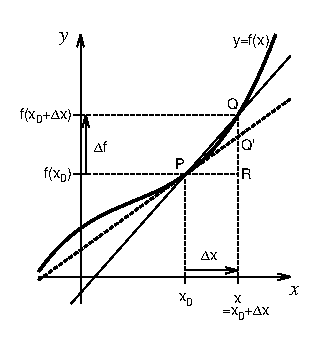
\includegraphics[width=7cm]{diff_explain.eps}
    \caption{関数$y=f(x)$のグラフ(太い実線)と, 点Pにおける接線のグラフ
(太い点線), そして$y=f(x)$上の2点P, Qを通る直線(細い実線)のグラフ。なお, 
原点$O$はどこにあるか定かでない(というか問題にならない)のでこのグラフには
書き込んでいない。}
\label{fig:diff_explain}\end{figure}

ここで, 点Pにおける接線(点Pでこの関数に接する直線; 
\fref{fig:diff_explain}の太い点線)を考えよう。その傾きを$a$とすると, 
この接線は点P$(x_0, f(x_0))$を通る, 傾き$a$の直線なので, 
その関数は$y=f(x_0)+a(x-x_0)$となる。

さて, もし$x_0$と$x$との間隔が十分に狭ければ, そのあたりでは, 
この関数のグラフ(\fref{fig:diff_explain}の太い実線)は, 
点Pにおける接線(\fref{fig:diff_explain}の太い点線)でざっくりと
近似できるだろう。すなわち, 次式が成り立つだろう:
\begin{eqnarray}
f(x) \fallingdotseq f(x_0)+a(x-x_0)\label{eq:define_dif0}
\end{eqnarray}
ここで"$\fallingdotseq$"は, 「ほぼ等しい」「近似的に等しい」という
意味の記号だ。\eref{eq:define_dif0}の左辺は点Qの$y$座標で, 
右辺は点Q'の$y$座標だ。点Qと点Q'は微妙にズレているので, 
=でなく$\fallingdotseq$と書くのだ。

先回りしてざっくり言えば, 微分というのは, この定数$a$
(接線の傾き)のことだ。でも, そこには深くて微妙な話があるので, 
しばらく辛抱して続きを読んで欲しい。

慣習的に, $x-x_0$を$\Delta x$と書く。$\Delta x$は
\fref{fig:diff_explain}のPRの長さである\footnote{ただしRがPの
左側にあるときはマイナスになる。}($\Delta$は\pref{q:logic_Greece}で学んだ
「デルタ」の大文字で, $\Delta$と$x$は別々の数
ではなく, "$\Delta x$"でひとつの数を表す)。そうすると, 
\begin{eqnarray}x=x_0+\Delta x\label{eq:define_dif_deltax}\end{eqnarray}
となる。\eref{eq:define_dif_deltax}を使うと, \eref{eq:define_dif0}は, 次のようになる:
\begin{eqnarray}
f(x_0+\Delta x) \fallingdotseq f(x_0)+a\Delta x\label{eq:define_dif0001}
\end{eqnarray}

さて, $x$を$x_0$に限りなく近づければ(それは\fref{fig:diff_explain}でRをPに近づけることに
相当し, それに伴って点Qや点Q'も点Pに近づいていく), $\Delta x$は限りなく0に
近づくだろう。究極的には$\Delta x$は0になってしまいそうなのだが, その寸前
で踏みとどまって, 「0ではないけれど, 限りなく0に近い」
という状態(極限)\index{きょくげん@極限}を想定する。そのときの$\Delta x$を, 
慣習的に$dx$と書く\footnote{$d$と$x$は別々の数ではなく, 
"$dx$"でひとつの数を表している。}。この場合, \eref{eq:define_dif0001}は, 以下のようになる:
\begin{eqnarray}
f(x_0+dx) = f(x_0)+a\,dx\label{eq:define_dif002}
\end{eqnarray}
ここで, もともと"$\fallingdotseq$"だったところが"$=$"に変わってしまった
ことに注意しよう。というのも, $\Delta x$が0に近づくとき, \fref{fig:diff_explain}
では, 点Qと点Q'が, 点Pでガチャンとぶつかりそうになるのでなく, 互いに寄り沿いながら
点Pに向かって行く。だから, \eref{eq:define_dif0001}の左辺と右辺の
誤差は, $\Delta x$が0に近づくよりもずっと速く0に近づく。
なので極限では, 誤差は実質的に0になる, つまり"$\fallingdotseq$"だったところ
を"$=$"と書いてよい, と考えるのだ\footnote{ただし, このあたり, 
厳密には論理的に微妙なことが多い。しかし初学者は, とりあえず
$\Delta x$と$dx$や, この後に出てくる$\Delta f$と$df$は, それぞれ互いに「同じようなもの」と思って
おいてよい。形式的には, 極限では$\Delta$が$d$になり, $\fallingdotseq$が$=$になるのだ。}。

この「限りなく0に近いけど0じゃない」というのは, 一種, 仮想的な状態である。その仮想的な微小量
$dx$を, \underline{無限小} \index{むげんしょう@無限小}
% (infinitesimal)
という。実際は, 0でない数は, 0との間に必ず有限な差が存在する。
そのような現実の微小量を\underline{有限小}\index{ゆうげんしょう@有限小}
という。上で書いた$\Delta x$が, 有限小である。
ちなみに, $dx$や$\Delta x$の"$d$"や"$\Delta$"は, "difference"
を意味する\footnote{ギリシャ文字の$\Delta$は, 由来としては英語のDに相当する。}。つまり
「差」とか「違い」である。$x=x_0$から「わずかに違うところ」として$x=x_0+dx$とか$x=x_0+\Delta x$
に着目するのだ。

さて, \eref{eq:define_dif002}で, 定数$a$を$f'(x_0)$と書く。これを
$f(x)$の$x=x_0$における\underline{微分係数} 
\index{びぶんけいすう@微分係数}と定義する。すなわち, 
\begin{itembox}{微分係数の定義(1)}
関数$f(x)$と微小量$dx$に関して, 次式を満たす数$f'(x_0)$を, $x=x_0$における
$f(x)$の微分係数と定義する:
\begin{eqnarray}
f(x_0+dx) = f(x_0)+f'(x_0)dx \label{eq:define_dif}
\end{eqnarray}
\end{itembox}
これを使えば\eref{eq:define_dif0001}は次のように書ける:
\begin{eqnarray}
f(x_0+\Delta x) \fallingdotseq f(x_0)+f'(x_0)\Delta x\label{eq:define_dif_Delta}
\end{eqnarray}
この式も, 後々, 重要になってくる。\mv

さて, 高校数学や数学類的な大学数学では, \eref{eq:define_dif}とはちょっと
違うスタイルで微分係数を定義する。それも説明しておこう。
\eref{eq:define_dif}を少し変形すると, 
\begin{eqnarray}
f'(x_0) = \frac{f(x_0+dx)-f(x_0)}{dx}\label{eq:define_dif10}
\end{eqnarray}
となる。あるいは, 有限小で書けば, 
\begin{eqnarray}
f'(x_0) \fallingdotseq \frac{f(x_0+\Delta x)-f(x_0)}{\Delta x}\label{eq:define_dif11}
\end{eqnarray}
となる。ここで, $\Delta x$が限りなく0に近づく極限を以下のように書く:
\begin{itembox}{微分係数の定義(2)}
\begin{eqnarray}
f'(x_0) :=\lim_{\Delta x \rightarrow 0} \frac{f(x_0+\Delta x)-f(x_0)}{\Delta x}\label{eq:define_dif2}
\end{eqnarray}
\end{itembox}
ここで極限では$\fallingdotseq$が$=$になったかわりに, 
「極限である」ということを忘れないように, "lim"という記号(\pref{eq:limit_new}で出てきた!)を前につけた。
$dx$という記号を使うなら, "lim"は不要である。
\eref{eq:define_dif2}は, 高校数学の教科書に載っている, 微分係数の定義である (
高校教科書では$\Delta x$のかわりに$h$という記号が使われるのが普通)。

微分係数の定義として, 
\eref{eq:define_dif}と, \eref{eq:define_dif2}は, 同じである。
これらの2つの式を, 必ず記憶しよう。でなければ, ここから先の数学を学ぶのは無駄だよ!

\begin{q}\label{q:diff_def00} \eref{eq:define_dif}と\eref{eq:define_dif2}を
それぞれ10回ずつ書いて記憶せよ。\end{q}

\begin{faq}{\small\textgt{10回ずつ書くなんてダルいです。}
... そうでもしないと, 覚えてくれない人が多くてね...}\end{faq}

\begin{faq}{\small\textgt{微分係数の定義が覚えられません。}
... 10回書いた? それでダメなら20回ね。}\end{faq}

\begin{faq}{\small\textgt{微分って, もっと難しいことかと思ったら, 出てくるのは
直線の式とか傾きとかだけですね}
 ... そうです。微分のアイデアはシンプル。直線(1次関数)を中学高校で
さんざん勉強したのは, 微分を理解する為でもあったのです。}\end{faq}

\begin{q}\label{q:diff_def0} 関数$g(x)$の, $x=a$における微分係数の定義を述べよ。\end{q}

%\begin{faq}{\small\textgt{この問題で, 「$g(a+dx)=g(a)+g'(a)dx$」と回答したら不正解になりました。
%なぜ? 式は合ってますよね?} ... $g(a)$や$dx$とは何か? その式のうちどの部分が微分係数か? 
%そういうことも書かないとダメ。式だけでなく, 式の中身を説明する文章も, 定義の一部なのです。}\end{faq}

さて, $f(x_0+dx)$や$f(x_0+\Delta x)$も, $f(x_0)$からみれば「わずかに違う」値であるので, 
これらと$f(x_0)$との差を, それぞれ$df$や$\Delta f$と書こう。すなわち, 
\begin{eqnarray}
&&df:=f(x_0+dx)-f(x_0)\label{eq:diff_def_df}\\
&&\Delta f:=f(x_0+\Delta x)-f(x_0)
\end{eqnarray}
と定義する。$\Delta f$は\fref{fig:diff_explain}での線分RQである
\footnote{ただしQがRより下にあるときはマイナスになる。}。
$df$とか$\Delta f$と書いてしまうと, なんだか独立した量のように見えてしまうが, 
定義から明らかなように, $df$は$dx$と, $\Delta f$は$\Delta x$と, それぞれ連動している。
すると, \eref{eq:define_dif}より, $f(x_0+dx)-f(x_0)=f'(x_0)dx$, つまり, 
\begin{eqnarray}
df=f'(x_0)dx\label{eq:define_dif001}
\end{eqnarray}
と書ける(\eref{eq:define_dif}の右辺の$f(x_0)$を左辺に移項して\eref{eq:diff_def_df}を使った)。
この\eref{eq:define_dif001}が表すのは, 「微小量どうしは比例する」という考え方である。
関数$f(x)$が複雑な関数であっても, 微小量で考えるとそれは一次関数になり, 
微小な差どうし($df$と$dx$)は比例関係になり, その比例係数が微分係数なのだ。

一次関数や比例関係はシンプルだから扱いやすいので, 難しい問題も, 
一次関数や比例関係の話に持ち込めばなんとかなる。そうするための
武器が微分である。

\begin{faq}{\small\textgt{一次関数や比例関係で表すことのメリット
がよくわかりません} ... もう少し辛抱してください。後に「積分」を学ぶと, 
それがわかります。微分と積分はセットの考え方なのです。}\end{faq}

また, \eref{eq:define_dif10}, \eref{eq:define_dif11}, \eref{eq:define_dif2}は, それぞれ
以下のようにも書ける:
\begin{eqnarray}
&&f'(x_0)=\frac{df}{dx}\label{eq:define_dif25}\\
&&f'(x_0)\fallingdotseq \frac{\Delta f}{\Delta x}\label{eq:define_dif3}\\
&&f'(x_0)=\lim_{\Delta x \rightarrow 0} \frac{\Delta f}{\Delta x}\label{eq:define_dif4}
\end{eqnarray}
特に\eref{eq:define_dif25}の書き方はよく出てくる。この右辺を
\begin{eqnarray}
\frac{d}{dx}f\label{eq:define_dif45}
\end{eqnarray}
と書くこともある。

\eref{eq:define_dif25}や\eref{eq:define_dif3}から明らかなように, 
$f(x)$に関する「わずかな違い」である$df$や$\Delta f$と, 
$x$に関する「わずかな違い」である$dx$や$\Delta x$との比(の極限)が, 微分係数である。
それは, \fref{fig:diff_explain}で言えば, 線分RQを線分PR
で割ったもの, すなわち「縦方向の違い」を「横方向の違い」で割ったもの, すなわち, 
「直線PQの傾き」である。それは接線(直線PQ')の傾き(RQ'/PR)とは微妙に違う。
しかし, $\Delta x$が十分に0に近ければ(Rが十分にPに近ければ), 
点Qは点Q'にすっと寄り添うように近づき, 直線PQと直線PQ'はほぼ重なるので, 
直線PQの傾きは接線の傾きに等しくなる, と考えるのだ。\\

さて, ここまでグラフのイメージを借りながら, 微分の発想と定義を説明した。
しかしここで強調したいことがある。それは「グラフのイメージに頼りすぎるな」
ということである。微分の本質は, その定義である\eref{eq:define_dif}や, 
\eref{eq:define_dif2}に全て込められている。それらは数式だけで
組み立てられており, グラフからイメージされる「接線の傾き」のような
言葉は全く出て来ていない。要するに, グラフは話をわかりやすくするため
だけで, 本当は\textgt{グラフなんか無くてもかまわない}のだ。でも, 
初学者がいきなり\eref{eq:define_dif}と, \eref{eq:define_dif2}
だけで「これが微分係数だ!」と教えられても, 
理解できないから数学が嫌いになってしまう。それを避けるためにグラフを使ったのだ。

\begin{faq}{\small\textgt{グラフは無意味ってことですか?} ... 
無意味とは言いません。グラフは, 何かのアイデアの種を探したり, 
アイデアを組み立てたり, それを人に伝えるには有用ですしね。でも, 
グラフにとらわれ過ぎると, 発想が限定されてしまうのです。
自転車の「補助輪」のようなものでしょうか。いずれはそれ無しで
走れるようになるのが理想です。

\begin{comment}
\textgt{なんか無茶苦茶なことを言われている気がしますが。}
... そうでしょう。でも, \eref{eq:define_dif}と\eref{eq:define_dif2}に
余計な意味やイメージを貼り付けると, それらの\textgt{切れ味が鈍る}
のです。大学では, グラフが描けないような関数, 例えば複素数を値にとるような関数や, 
複数の変数を持つような関数の微分も考えます。そういうときは, \fref{fig:diff_explain}
のようなグラフはイメージできないから, グラフやイメージに頼った「意味」は
無意味になります。でも, たとえグラフが描けなくても和・差・積・商ができる対象
(例えば複素数)なら, \eref{eq:define_dif}と\eref{eq:define_dif2}
は意味を持つので, 微分はできます。\eref{eq:define_dif}は
商(割り算)すら使っていないので, 和・差・積はできるけど商はできないような
対象(後で学ぶベクトルや行列など)も\eref{eq:define_dif}で微分できる
のです。また, これから微分に関する様々な定理(公式)を証明していきますが, 
そこでもグラフはほとんど出て来ないし, 役に立ちません。
\eref{eq:define_dif}か\eref{eq:define_dif2}があれば十分なのです。\\

\textgt{でも, イメージが湧かないとわからないし受け入れられないですよ}
... それが悲しいところです。我々はどうしてもイメージや意味を求めてしまう。
そこに数学の勉強の苦しさがあるのです。大学の数学は, 我々の日常感覚の
延長ではイメージできないし意味もわからないものまで相手にします。
イメージや意味を性急に求める人は, 低レベルの数学から先には行けません。
まずは素直に定義を受け入れ, 論理を追いかけ, 例を考えるのです。
そうすればイメージが湧いてくるのです。\\

\textgt{低レベルの数学から先に行けなくてもいいです}
 ... もったいない! この先, すんごい綺麗で強力な数学があるのに...\\
\end{comment}
\textgt{結局, 「微分とは接線の傾きである」と言ったら
ダメなんですか?} ... 「定義」としてはダメ
です。数学の論理では, そもそも「接線」の定義に微分が必要なのです。
「イメージ」としても, あえてグラフに頼らずに「微小量どうしの
比例関係の比例係数」と考える方が, 後々, 便利です。無論, それは
グラフで描けば「接線の傾き」ですが, グラフが描けない状況でも使えます。

\textgt{微分と微分係数は同じもの?} ... このへんは微妙で, 
同じものを指すことが多いです。本来は, 微分とは, $dx$や$df$などの微小量
のことで, 微分係数は微小量同士の比例係数$f'(x_0)$です。でも, 
多くの本では, 微分係数や, このあと学ぶ導関数のことを「微分」と
言います。特に, 「微分せよ」という指示は, ほぼ間違いなく, 微分係数や
導関数を求めよという意味です。}\end{faq}

\begin{comment}
\begin{faq}{\small\textgt{複素数は複素平面に描けるから, 複素数の関数の
グラフも描けるんじゃないでしょうか?} ... $y=f(x)$の
$x$と$y$が複素数なら, $x$は実部と虚部という2つの実数を含んでるし, 
$y$も同様。つまり2つの実数を与えて2つの実数が返される関数だから, 
そのグラフには全部で4つの座標軸が必要です。あなたは4次元空間を想像できますか?}\end{faq}
\end{comment}

さて, 関数$f(x)$の, 様々な点における微分係数を集めてならべた関数
を\underline{導関数} (derivative)\index{どうかんすう@導関数}
と呼び, $f'(x)$と書く。微分係数や導関数を求めることを「微分する」(differentiate)と言う。

では具体的にいくつかの関数を微分してみよう。以後, 簡単のため, 定義\eref{eq:define_dif}の
$x_0$を$x$と書き直す。\mv

\begin{exmpl} 関数$f(x)=2x+1$を微分してみよう:
\begin{eqnarray*}
f(x+dx)&=&2(x+dx)+1\\
&=&2x+1+2dx\\
&=&f(x)+2dx
\end{eqnarray*}
\eref{eq:define_dif}と較べると, $dx$の係数が導関数$f'(x)$だから, 
\begin{eqnarray}f'(x)=2\label{eq:diff_2x_1}\end{eqnarray}
となる。(例おわり)\end{exmpl}

\eref{eq:diff_2x_1}は, 以下のようにも書く:
\begin{eqnarray}(2x+1)'=2\label{eq:diff_2x_12}\end{eqnarray}
\eref{eq:diff_2x_12}の左辺のように, 何かの関数の微分(導関数)を表すには, 
その関数をカッコ( )で囲って, ダッシュ(')をつける。あるいは, 
\begin{eqnarray}\frac{d}{dx}(2x+1)=2\label{eq:diff_2x_13}\end{eqnarray}
のように, 微分したい関数の前に$d/dx$という記号を書いてもよい。

\begin{faq}{\small\textgt{導関数と微分係数の違いがよくわかりません。}
... 導関数は関数。その1箇所での値が微分係数。たとえば例\ref{ex:x2deriv}で
学ぶように, $f(x)=x^2$という関数の導関数は$f'(x)=2x$。そいつの$x=3$での
値$f'(3)=6$が, 「$x=3$における微分係数」です。}\end{faq}

\begin{q}\label{q:diff_const} $p, q$を任意の定数とする。一次関数$f(x)=px+q$を微分すると, $f'(x)=p$となること, つまり
\begin{eqnarray}(px+q)'=p\label{eq:diff_px+q}\end{eqnarray}
を示せ。特に, 定数関数$y=q$を微分すると, 恒等的に0になること, つまり
\begin{eqnarray}(q)'=0\label{eq:diff_q}\end{eqnarray}
を示せ。\end{q}
\mv


定数関数のグラフは, $x$軸と平行な直線なので, どの場所でも傾きは0である。そのことからも, 
定数関数の導関数が恒等的に0であることが納得できるだろう。

また, 一次関数$px+q$のグラフは, 切片$q$, 傾き$p$の直線である。従って, どの場所でも
傾きは$p$である。そのことからも, $px+q$の導関数が恒等的に$p$であることが納得できるだろう。

\begin{exmpl}\label{ex:x2deriv} 関数$f(x)=x^2$を微分してみよう。
\begin{eqnarray*}
f(x+dx) & = & (x+dx)^2\\
        & = & x^2+2x\,dx +dx^2\\
        & = & f(x)+2x\,dx +dx^2
\end{eqnarray*}
ここで, $dx^2$は, $d\times x^2$ではなく, $(dx)^2$である。というのも, 
既に述べたように, $dx$は$d\times x$ではなく$dx$のひとまとまりでひとつの数(微小量)を
表すからだ。さて, $dx$は0に
近い量なので, \textgt{その2乗である$dx^2$は, さらに, はてしなく0に
近いはずだ。そこで, この$dx^2$の項は無視しよう!} そうすると, 
\begin{eqnarray}f(x+dx)=f(x)+2xdx\end{eqnarray}
となる。\eref{eq:define_dif}と較べると, $dx$の係数は$2x$だから, $f'(x)=2x$となる。(例おわり)\end{exmpl}
\hv

この例の\textgt{$dx^2$は無視する}という考え方は極めて重要である。換言すれば, 
「$\Delta x$は無視できないが$\Delta x^2$は無視できる」くらいに$\Delta x$が0に
近づく状況が, これまで述べてきた「$\Delta x$が限りなく0に近づく」ということ, つまり
「$\Delta x$が$dx$になること」, つまり「極限」の, 具体的な意味である。そのような状況では, 
多くの関数で, $\Delta f$と$\Delta x$が, 単なる比例関係になる(とみなせる)。
その比例係数が微分係数(または導関数)である。\mv

\begin{faq}{\small \textgt{「微分する」って, 要するに$dx$の比例係数を求めること?}
... ざっくりいえばそういうことです。関数を$dx$の1次関数で近似したときの, 
$dx$の比例係数を求めることです。中学校であんなに比例とか
1次関数をさんざん勉強させられたのは, この伏線だったのです。}\end{faq}

\begin{faq}{\small\textgt{高校で「微分係数」を習った時は, 
一体どこが係数なのかと思っていましたが, 本当に係数だったのですね}
... そうなんです。$dx$の係数が「微分係数」です。その発想を足がかりに, 
本書の後半では, 微分をもっと広く拡張していきます。}\end{faq}

\begin{faq}{\small\textgt{$dx^2$を0とする, 等の基準がわからなくて
使うのがこわいです} ... $dx$と$dx^2$が混在している時は, $dx^2$は$dx$
よりはるかに小さいので無視する, ということです。
もし$dx$が0.01なら$dx^2$は0.0001になり、$dx$よりもはるかに
小さいですよね($dx$は限りなく0に近い微小量なので, このように
具体的な値を例に挙げるのは本当は間違っているのですが)。
}\end{faq}

\begin{exmpl} 関数$f(x)=x^n$を微分してみよう($n$は1以上の整数の定数)。
二項定理(P.\pageref{eq:binomth2}の\eref{eq:binomth2})より, 
\begin{eqnarray}
&&f(x+dx)=(x+dx)^n\nonumber\\
&&=_n\text{C}_0x^n+_n\text{C}_1x^{n-1}dx +_n\text{C}_2x^{n-2}dx^2+\cdots\nonumber\\
&&=x^n+nx^{n-1}dx +_n\text{C}_2x^{n-2}dx^2+\cdots\nonumber\\
&&=f(x)+nx^{n-1}dx +_n\text{C}_2x^{n-2}dx^2+\cdots
\end{eqnarray}
ここで$dx^2$以降の項は無視。\eref{eq:define_dif}と較べると, $dx$の係数は$nx^{n-1}$だから, 
\begin{eqnarray}
f'(x)=nx^{n-1}\label{eq:diff_x}
\end{eqnarray}となる。(例おわり)\end{exmpl}
\hv

\begin{exmpl}\label{ex:1overxderiv} 関数$f(x)=1/x$を微分してみよう。まず, 
\begin{eqnarray}f(x+dx)=\frac{1}{x+dx}\end{eqnarray}
ここで, 分子と分母の両方に$x-dx$を掛けると, 
\begin{eqnarray}
f(x+dx)&=&\frac{x-dx}{(x+dx)(x-dx)}\nonumber\\
      &=&\frac{x-dx}{x^2-dx^2}
\end{eqnarray}
ここで, 分母の$dx^2$を無視すると, 
\begin{eqnarray}
f(x+dx)&=& \frac{x-dx}{x^2}\nonumber\\
      &=&\frac{1}{x}-\frac{1}{x^2}dx\nonumber\\
      &=&f(x)-\frac{1}{x^2}dx
\end{eqnarray}
\eref{eq:define_dif}と較べると, $dx$の係数は$-1/x^2$だから, 
\begin{eqnarray}
f'(x)=-\frac{1}{x^2}\label{eq:dif_recipr}
\end{eqnarray}
ところでこれは, \eref{eq:diff_x}で$n=-1$とおいた場合に一致する。
もともと\eref{eq:diff_x}では, 定数$n$を$1$以上の整数としたが, $n=-1$の
ときも成り立つことがわかった。
(例おわり)\end{exmpl}
\vv



\section{数値微分}\label{sect:numdiff}

これから具体的に関数を微分する方法を学ぶのだが, まず, 
計算機で微分するやり方を学ぼう。それを
「\underline{数値微分}」 \index{すうちびぶん@数値微分}という。
数値微分は原理が単純で, 微分のアイデアを理解するのに
良い題材だ。また, 実際に世の中で数値微分は様々な場で使われている。
というわけで, 微分の勉強はまず計算機から入るのだ。

\eref{eq:define_dif2}で学んだように, 微分は次式で定義される:
\begin{equation}f'(x):=\lim_{\Delta x \to 0}\frac{f(x+\Delta x)-f(x)}{\Delta x}\end{equation}

実際は, $\Delta x$が「限りなく0に近く」なくても, ある程度まで0に近づければ, このリミットを無視しても, 
そこそこ正確に計算できるだろう:
\begin{equation}
f'(x)\fallingdotseq \frac{f(x+\Delta x)-f(x)}{\Delta x}\label{eq:PC_diff0}
\end{equation}
これが, 計算機に微分をやらせるときの考え方である。すなわち, 
$f(x)$について隣り合うセルどうしの引き算をして($f(x+\Delta x)-f(x)$), それを$x$について隣り合う
セルどうしの引き算(つまり$\Delta x$, つまり刻み幅)で割ればよい。

例えば$f(x)=x^2$を微分してみよう。スプレッドシートで, $x$の値を$-1$から1まで0.05刻みで
A列に与え, $f(x)$の値をB列に与える:\\
\begin{tabular}{|>{\columncolor[gray]{0.8}}c|c|c|c|} \hline
\rowcolor[gray]{0.8} & A & B & C \\ \hline
1 & x & f(x)=x^2 & f'(x) \\ \hline
2 & -1    & 1 &  \\ \hline
3 & -0.95 & 0.9025 &  \\ \hline
4 & -0.9  & 0.81 &  \\ \hline
5 & -0.85 & 0.7225 &  \\ \hline
$\cdots$ & $\cdots$ & $\cdots$ &  \\ \hline
\end{tabular}\\

ここで右端の列(C列)で微分$f'(x)$を計算するには, セルC2に, 「=(B3$-$B2)/(A3$-$A2)」という式を
書き込む。ここでB3$-$B2というのは$f(x+\Delta x)-f(x)$に相当し, A3$-$A2というのが$\Delta x$に
相当する。厳密には, このような計算式で与えられる微分の値(つまり微分係数)
は, $x=-1$のときではなく, $x=-1$と$x=-0.95$の中間付近だが, どうせ$x$の
刻み($\Delta x=0.05$)は小さいから, あまり気にしない。気になるなら, 
刻みをもっと小さくとればよい。

そして, C2セルの内容を, C3以降のC列全体にコピーペーストすれば, C列に, 
近似的ではあるが, $f'(x)$ができあがる。こうして計算機で関数の微分を
近似的に行うことを, \underline{数値微分} \index{すうちびぶん@数値微分}と呼ぶ。\hv

\begin{q}\label{q:comp_diff0} 表計算ソフト, 関数$f(x)=x^2$を, $-1 \le x \le 1$
の範囲で数値微分し, その結果を, $f(x)$と, 解析的\footnote{理論的に厳密な計算(式変形)で答えを導く
ことを\underline{解析的}\index{かいせきてき@解析的}という。「数値的」の対義語である。}
な微分結果$f'(x)=2x$とともに, グラフに描いてプリントアウトせよ。$\Delta x$は各自で適当に定めよ。
結果は\fref{fig:diffx2}のようになるはず!
\end{q}
\begin{figure}[!h]
    \centering
    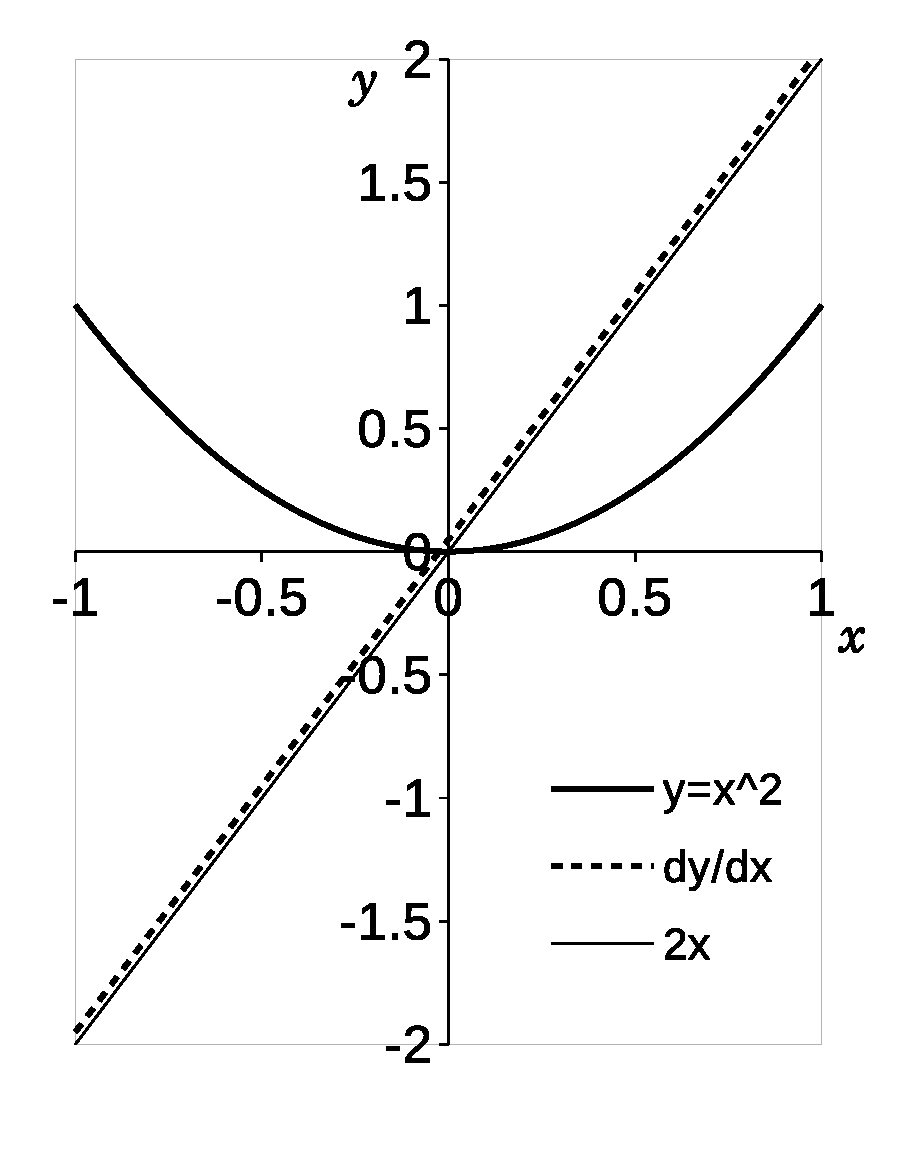
\includegraphics[width=4.7cm]{diffx2.eps}
    \caption{$y=x^2$とその数値微分($dy/dx$), そして$y=2x$。$x$の刻みは0.05。
数値微分と$y=2x$は, 刻みを小さくすればもっと近くなる。
例\ref{ex:x2deriv}の結論を数値微分でも確認できた!\label{fig:diffx2}}
\end{figure}
\hv


\section{グラフから導関数を直感的に作る}

導関数という概念を, グラフでもう少し直感的に考えてみよう。例として図\ref{fig:diff_graph}を
考える。ここには, ある関数$y=f(x)$と(上段), その導関数$y=f'(x)$ (下段)のそれぞれのグラフ
を上下に並べて描いてある。$y=f(x)$のグラフ上の点A, B, C, D, Eを考えよう。各点における
接線を, 点線で描いてある。これらの接線は, 点Aや点Eではほどんど水平だが, 点B, C, Dでは
右上がりである。特に, 点Cでの接線はかなり急な傾きを持っている。

従って, 「接線の傾き」という観点では, 点A, Eではほぼ0であり, 点B, Dでは「そこそこ」の大きさ, 
そして点Cで最も大きい。直感的には, 「接線の傾き」は微分係数のことなので, 各点での
「接線の傾き」をグラフにすると, ひとつの山型のグラフができる。それが下段の$y=f'(x)$である。

\begin{figure}[!h]
    \centering
    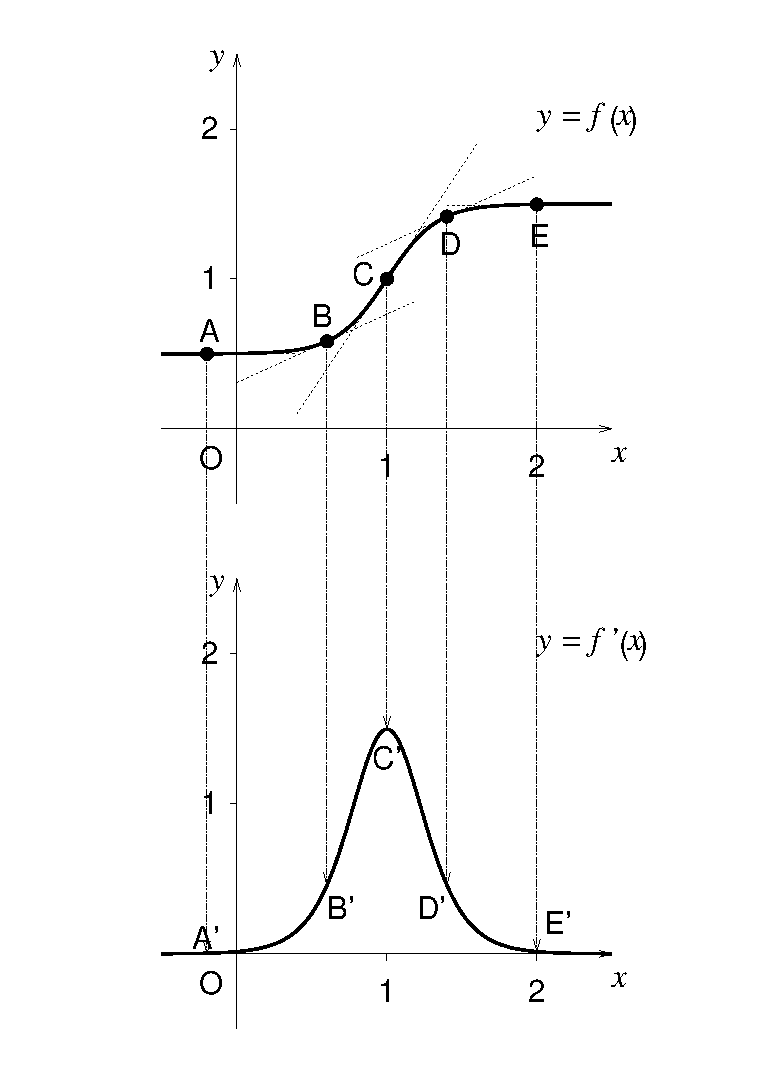
\includegraphics[width=8cm]{diff_graph.eps}
    \caption{関数$y=f(x)$とその導関数$y=f'(x)$。
$y=f(x)$のグラフは点C付近で傾き最大。従って, そのとき
導関数$y=f'(x)$は最大値をとる(点C')。\label{fig:diff_graph}}
\end{figure}

このように考えれば, 関数を数式として与えられなくても, その関数のグラフが与えられれば, 
その関数の導関数のグラフの概形を直感的に描くことができる。すなわち, 
関数上のいくつかの点での「接線の傾き」を考えて, それを別のグラフにプロットすれば
よいのだ。

\begin{q}\label{q:diff_graph_ex} 図\ref{fig:diff_graph_ex}に
に描かれた2つの関数について, それぞれ導関数の概形を重ねて描け。レポートを書くときは, 
レポート用紙にまずこのグラフを写しとってから, それに重ねて描け。
\end{q}
\begin{figure}[!h]
    \centering
    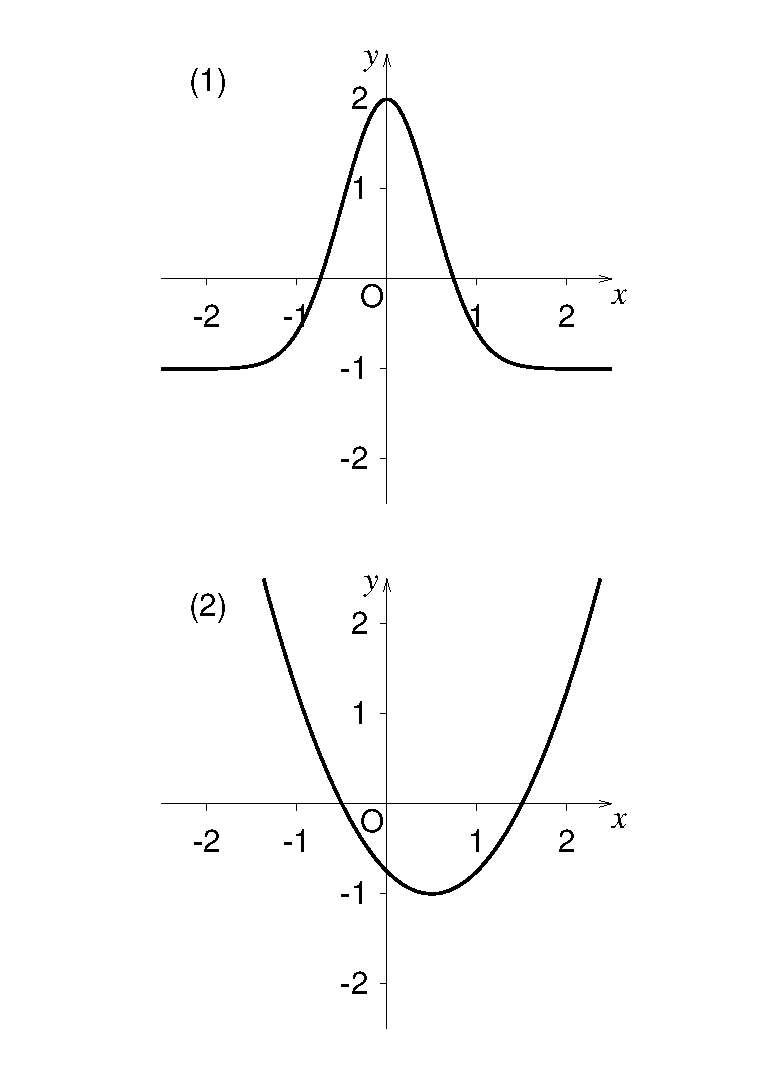
\includegraphics[width=8cm]{diff_graph_ex.eps}
    \caption{問\ref{q:diff_graph_ex}のグラフ。それぞれの導関数の概形を
描いてみよう。(1)のヒント: 左右の端と中央($x=0$)で, 接線の傾きは0になる。$x<0$では
右上がりなので接線の傾きはプラス。$0<x$では右下がりなので接線の傾きはマイナス。
\label{fig:diff_graph_ex}}
\end{figure}
\hv


\section{微分の公式}\label{sect:diff_formula}

実際に関数を微分するときは, 微分係数(導関数)の定義\eref{eq:define_dif}に
遡ってやることは少ない。複雑な関数の場合は前節でやったように数値微分を使うし, 
そうでなければ, 以下に示すような, いくつかの便利な定理(公式)を活用して
ちゃっちゃとやってしまうのだ。以下, $f(x), g(x)$を, 任意の(微分可能な)関数とする。
\hv

\begin{itembox}{微分の公式1: 足し算はバラせる}
\begin{eqnarray}
\{f(x)+g(x)\}'=f'(x)+g'(x)\label{eq:diff_form1}
\end{eqnarray}
\end{itembox}
証明: $F(x)=f(x)+g(x)$とおくと, 
\begin{eqnarray}
F(x+dx) & = & f(x+dx)+g(x+dx)\nonumber\\
               & = & f(x)+f'(x)dx+g(x)+g'(x)dx\nonumber\\
               & = & f(x)+g(x)+\{f'(x)+g'(x)\}dx\nonumber\\
               & = & F(x)+\{f'(x)+g'(x)\}dx
\end{eqnarray}
ここで, $dx$の係数に着目すると, 微分係数の定義から, $F'(x)=f'(x)+g'(x)$。\qed
\vv

\begin{exmpl}  $f(x)=x^2+2x$を微分しよう。公式1を使うと, 
\begin{eqnarray}
f'(x)=(x^2+2x)'=(x^2)'+(2x)'
\end{eqnarray}
となる。例\ref{ex:x2deriv}から, $(x^2)'=2x$であり,\eref{eq:diff_px+q}から, $(2x)'=2$である。従って, 
\begin{eqnarray}
f'(x)=2x+2
\end{eqnarray}
となる。(例おわり)\end{exmpl}
\hv

\begin{itembox}{微分の公式2: 定数倍は前に出せる}
$a$を定数として, 
\begin{eqnarray}
\{af(x)\}'=af'(x)\label{eq:diff_form2}
\end{eqnarray}
\end{itembox}
証明: $F(x)=af(x)$とおくと, 
\begin{eqnarray}
F(x+dx) & = & af(x+dx) = a\{f(x)+f'(x)dx\}\nonumber\\
               & = & af(x)+af'(x)dx\nonumber\\
               & = & F(x)+af'(x)dx
\end{eqnarray}
ここで, $dx$の係数に着目すると, 微分係数の定義から, $F'(x)=af'(x)$。\qed
\hv

微分の公式1と2のような性質は, 数列の和$\Sigma$にもあった
こと(P.\pageref{eq:sum_linear1})を覚えているだろうか? (線型性)\hv

\begin{exmpl}  $f(x)=3x^2$を微分しよう。公式2を使うと, 
\begin{eqnarray}
f'(x)=(3x^2)'=3(x^2)'
\end{eqnarray}
となる。例\ref{ex:x2deriv}から, $(x^2)'=2x$である。従って, 
\begin{eqnarray}
f'(x)=3(2x)=6x
\end{eqnarray}
となる。(例おわり)\end{exmpl}\

\begin{exmpl} 関数$f(x)=x^3+2x^2+3x+1$を微分しよう。
公式1, 公式2より, 
\begin{eqnarray}f'(x)=(x^3)'+2(x^2)'+3(x)'+(1)'\end{eqnarray}
ここで, 右辺の$(1)'$とは定数関数1(すべての$x$に対して定数1を対応させる関数)の微分であり, 
\eref{eq:diff_q}より, もちろん0である。$(x^3)'$や$(x^2)'$, $(x)'$に
\eref{eq:diff_x}を使うと, 
\begin{eqnarray}=3x^2+4x+3\end{eqnarray}
(例おわり)\end{exmpl}
\hv

%-----------

\begin{q}\label{q:diff_func0} 以下の関数を微分せよ:
\begin{enumerate}
\item $f(x)=x^2+x+1$
\item $f(x)=4x^2+5x+6$
\item $f(x)=3x^2+3x+4$
\item $f(x)=5/x$ (ヒント: 例\ref{ex:1overxderiv}を使う)
\item $f(x)=x-1/x$
\end{enumerate}\end{q}
\hv

\begin{itembox}{微分の公式3: 積の微分}
\begin{eqnarray}
\{f(x)g(x)\}'=f'(x)g(x)+f(x)g'(x)\label{eq:diff_form3}
\end{eqnarray}
\end{itembox}

証明: $F(x)=f(x)g(x)$とおくと, 
\begin{eqnarray*}
F(x+dx) & = & f(x+dx)g(x+dx)\\
               & = & \{f(x)+f'(x)dx\}\{g(x)+g'(x)dx\}\\
               & = & f(x)g(x)+f'(x)g(x)dx\\
               &   & +f(x)g'(x)dx+f'(x)g'(x)dx^2
\end{eqnarray*}
ここで, $dx^2$を無視し, さらに, $dx$の項を整理し, また, $f(x)g(x)$を$F(x)$で置き換えると, 
\begin{eqnarray*}F(x+dx)= F(x)+\{f'(x)g(x)+f(x)g'(x)\}dx\end{eqnarray*}
$dx$の係数に着目すると, 微分係数の定義から, 
\begin{eqnarray}F'(x)=f'(x)g(x)+f(x)g'(x)\end{eqnarray}
\qed
\hv

\begin{exmpl}  関数$F(x)=(x^2+2)(x^2+x+3)$を微分しよう。
$f(x)=x^2+2$, $g(x)=x^2+x+3$として, 公式3を使うと, 
\begin{eqnarray}
F'(x)&=&(x^2+2)'(x^2+x+3)+(x^2+2)(x^2+x+3)'\nonumber\\
     &=&2x(x^2+x+3)+(x^2+2)(2x+1)\nonumber\\
     &=&4x^3+3x^2+10x+2
\end{eqnarray}
となる。一方, 先に因数を展開してしまって, 
\begin{eqnarray}
F'(x)&=&(x^4+x^3+5x^2+2x+6)'\nonumber\\
     &=&(x^4)'+(x^3)'+5(x^2)'+2(x)'+(6)'\nonumber\\
     &=&4x^3+3x^2+10x+2
\end{eqnarray}
とすることもできる。どちらのやりかたでやっても, 答えは一致する。このように, 
数学は色んなやり方で正解に到達できるものなのだ。
(例おわり)\end{exmpl}
\hv

%-----------
\begin{q}\label{q:diff_func1} 以下の関数:
\begin{eqnarray}f(x)=(x^2+x+1)(x^2-x-2)\end{eqnarray}
について, 
\begin{enumerate}
\item 2つの関数: $x^2+x+1$と$x^2-x-2$の積とみなして, 積の微分の公式を使って微分せよ。
\item 因数を展開して(つまり掛け算を実行してカッコを外して)から微分し, 前小問の結果と一致することを確認せよ。
\end{enumerate}\end{q}
\vspace{0.3cm}

「関数$f(x)$」などの$(x)$を省略して書くことがよくある。式が単純になって
見やすいし覚えやすい。公式1, 2, 3は, それぞれ以下のようになる:
\begin{eqnarray}
(f+g)'&=&f'+g'\\
(af)'&=&af'\\
(fg)'&=&f'g+fg'
\end{eqnarray}

さて, 多くの学生がつまずくのが次の公式である。といっても, しっかり説明を
読めば難しくないはずだ。

\begin{itembox}{微分の公式4: 合成関数の微分}
\begin{eqnarray}
\{g(f(x))\}'=g'(f(x))f'(x)\label{eq:diff_form4}
\end{eqnarray}
注: ここで$g'(f(x))$は, $g(x)$の導関数$g'(x)$の$x$の部分に$f(x)$を代入したもの
であり, $g(f(x))$の導関数ではない。\end{itembox}

証明の前に例を示す:

\begin{exmpl}\label{exmpl:bibun_x213}  関数$(x^2+1)^3$を微分しよう。この関数を, 
「$g(x)=x^3$という関数の$x$の部分に, $f(x)=x^2+1$という関数を入れたもの」
とみなす。$g'(x)=3x^2$だから, 公式4より, 
\begin{eqnarray}
\{(x^2+1)^3\}'&=&\{(f(x))^3\}'=3(f(x))^2f'(x)\nonumber\\
               &=&3(x^2+1)^2\,\{(x^2+1)'\}=3(x^2+1)^2(2x)\nonumber\\
               &=&6x(x^2+1)^2\label{eq:diffexample9}
\end{eqnarray}
となる。これで完了としてよいのだが, ここではあえて\eref{eq:diffexample9}を展開すると, 
\begin{eqnarray}
6x^5+12x^3+6x\label{eq:diffexample91}
\end{eqnarray}
となる。一方, $(x^2+1)^3$を先に展開してから微分すると,
\begin{eqnarray}
\{(x^2+1)^3\}'&=&(x^6+3x^4+3x^2+1)'\nonumber\\
               &=&6x^5+12x^3+6x\label{eq:diffexample92}
\end{eqnarray}
となる。\eref{eq:diffexample91}, \eref{eq:diffexample92}は一致している
(つじつま合っている)。(例おわり)\end{exmpl}

この例は別に公式4を使わなくても, 式を展開してから
普通に微分すれば解けた。しかし, 次の例のように, 公式4がどうしても
必要になる場面もたくさんある:\mv

\begin{exmpl} 次の関数を微分しよう。
\begin{eqnarray}\frac{1}{2x^2+1}\end{eqnarray}
$f(x)=2x^2+1$, $g(x)=1/x$として, 
公式4を使おう。\eref{eq:dif_recipr}より$g'(x)=-1/x^2$である。従って, 
\begin{eqnarray}
\Bigl\{\frac{1}{2x^2+1}\Bigr\}'
&=&-\frac{1}{(f(x))^2}\times f'(x)\nonumber\\
&=&-\frac{1}{(2x^2+1)^2}\times(2x^2+1)'\nonumber\\
     &=&-\frac{4x}{(2x^2+1)^2}\label{eq:diffexample95}
\end{eqnarray}
となる。(例おわり)\end{exmpl}
\mv

実際には, こういうふうに$g(x)$や$f(x)$をわざわざ
作ったりしないで, 頭の中でまず$2x^2+1$をひとつの
変数とみなして全体を微分し, さらに$2x^2+1$を$x$で微分して掛け合わせ, 
いきなり\eref{eq:diffexample95}の最後の行を暗算で導出
できるようになるのが望ましい。最初は難しいかもしれないが, 慣れるまで練習しよう。\hv

では公式4を証明しよう: $F(x)=g(f(x))$とおくと, 
\begin{eqnarray}
F(x+dx) & = & g(f(x+dx))\nonumber\\
        & = & g\bigl(f(x)+f'(x)dx\bigr)\label{eq:dif_gosei1}
\end{eqnarray}
ここで, $dx$は0に限りなく近い微小量なので, それに$f'(x)$を掛けた数, すなわち$f'(x)dx$も, 
0に限りなく近い微小量とみなすことができる。そこで, 微分係数の定義\eref{eq:define_dif}
において, $f(x)$を$g(x)$とし, $x_0$を$f(x)$とし, $dx$を$f'(x)dx$とすれば, 
\begin{eqnarray}
g\bigl(f(x)+f'(x)dx\bigr)= g(f(x))+g'(f(x))\{f'(x)dx\}\nonumber\\\label{eq:dif_gosei2}
\end{eqnarray}
となる。右辺第一項の$g(f(x))$は, もちろん$F(x)$である。従って, \eref{eq:dif_gosei1}\eref{eq:dif_gosei2}より, 
\begin{eqnarray}
F(x+dx)=F(x)+g'(f(x))f'(x)dx\label{eq:dif_gosei3}
\end{eqnarray}
$dx$の係数に着目すると, 微分係数の定義から, \\
$F'(x)=g'(f(x))f'(x)$。\qed
\vv

この公式は, 一見, 複雑そうに見えるが, \eref{eq:define_dif25}のような書き方を使うと,
\begin{eqnarray}
\frac{dg}{dx}=\frac{dg}{df}\frac{df}{dx}\label{eq:diff_form45}
\end{eqnarray}
と表せる。右辺に現れる2つの微分の掛け算を, 形式的に, 微小量$dg$, $df$, $dx$の
分数の掛け算とみなせば, 右辺を約分したものが左辺になるだけだ。\mv

%-----------
\begin{q}\label{q:diff_func2} 以下の関数を, 合成関数の微分の公式を使って微分せよ:
\begin{enumerate}
\item $F(x)=(3x^2+2)^3$
\item $F(x)=(x^2+x+1)^3$
\item $F(x)=(x^5+x^4+x^3+x^2+x+1)^2$
\item $F(x)=(1+1/x)^2$
\end{enumerate}\end{q}
\mv


%-----------
\begin{q}\label{q:diff_func3} 関数$u(x)$の逆数であらわされる関数$1/u(x)$の導関数は, 
以下で与えられることを示せ\footnote{\eref{eq:difdiv0}, \eref{eq:difdiv}では関数$u(x)$の「$(x)$」を
省略して書いていることに注意せよ。}:
\begin{eqnarray}
\Bigl(\frac{1}{u}\Bigr)'=-\frac{u'}{u^2}\label{eq:difdiv0}
\end{eqnarray}\end{q}
ヒント: $g(x)=1/x$, $f(x)=u(x)$として公式4を使う。
\mv

%-----------
\begin{q}\label{q:diff_func4} 関数$v(x)$と$u(x)$の比で作られる関数$v(x)/u(x)$の導関数は, 以下で与えられることを示せ:
\begin{eqnarray}
\Bigl(\frac{v}{u}\Bigr)'=\frac{v'u-vu'}{u^2}\label{eq:difdiv}
\end{eqnarray}\end{q}
\mv

%-----------
\begin{q}\label{q:diff_func5} 以下の関数を微分せよ:
\begin{edaenumerate}
\item \begin{eqnarray*}f(x)=\frac{1}{1+x^2}\end{eqnarray*}
\item \begin{eqnarray*}f(x)=\frac{x}{1+x^2}\end{eqnarray*}
\end{edaenumerate}
ヒント: (1)では$u(x)=1+x^2$として\eref{eq:difdiv0}を使う。(2)では$u(x)=1+x^2$, $v(x)=x$と
して\eref{eq:difdiv}を使う。
\end{q}
\mv

\begin{exmpl}  $1/x^n$を微分してみよう($n$は1以上の整数の定数とする)。この関数は, 
\begin{eqnarray*}g(x)=x^n\,\,\,\text{と, }f(x)=\frac{1}{x}\end{eqnarray*}
の合成関数とみなせる。実際
\begin{eqnarray}g(f(x))=\Bigl(\frac{1}{x}\Bigr)^n=\frac{1}{x^n}\end{eqnarray}
となる。ところで,\eref{eq:diff_x}より$g'(x)=nx^{n-1}$であり, 例\ref{ex:1overxderiv}より$f'(x)=-1/x^2$だから, 
\eref{eq:diff_form4}より, 次式が成り立つ:
\begin{eqnarray}
\Bigl(\frac{1}{x^n}\Bigr)'&=&n\Bigl(\frac{1}{x}\Bigr)^{n-1}\Bigl(\frac{1}{x}\Bigr)'\nonumber\\
     &=&n\Bigl(\frac{1}{x}\Bigr)^{n-1}\Bigl(-\frac{1}{x^2}\Bigr)\nonumber\\
     &=&-\frac{n}{x^{n+1}}
\label{eq:xpowminusn1}\end{eqnarray}
\end{exmpl}

\eref{eq:xpowminusn1}は次のように書き換えられる。
\begin{eqnarray}(x^{-n})'=\,-n\,x^{-n-1}\label{eq:xpowminusn3}\end{eqnarray}
これは, \eref{eq:diff_x}で$n$を$-n$と置き換えたものに一致する。
もともと\eref{eq:diff_x}では, $n$を$1$以上の整数としたが, これで, 
定数$n$が負の整数のときも成り立つことがわかった。\hv

次に学ぶ公式は, 公式4の応用だ。これは\pref{eq:taisuu00}で
学んだ対数を微分したりするのに使う(その話は後の章に出てくる)。

\begin{itembox}{微分の公式5: 逆関数の微分}
$g(x)$を$f(x)$の逆関数とすると
\begin{eqnarray}
g'(x)=\frac{1}{f'(g(x))}\label{eq:diff_form5}
\end{eqnarray}
注: ここで$f'(g(x))$は, $f(x)$の導関数$f'(x)$に
$g(x)$を代入したものだ。$f(g(x))$の導関数ではない。
\end{itembox}
証明: 
%\begin{eqnarray}
%&&f(x)=y\label{eq:diff_form5_p1}\\
%&&f(x+dx)=y+dy\label{eq:diff_form5_p2}
%\end{eqnarray}
%とする。$dx, dy$はともに微小量である。逆関数の定義より, 
%\begin{eqnarray}
%&&x=g(y)\label{eq:diff_form5_p3}\\
%&&x+dx=g(y+dy)\label{eq:diff_form5_p5}
%\end{eqnarray}
%である。\eref{eq:diff_form5_p3}, \eref{eq:diff_form5_p5}より, 
%\begin{eqnarray}dx=g(y+dy)-g(y)\label{eq:diff_form5_p7}\end{eqnarray}
%である。さて, $f(x)$の導関数の定義式:
%\begin{eqnarray}f(x+dx) = f(x)+f'(x)dx\label{eq:diff_form5_p8}\end{eqnarray}を考える。左辺は\eref{eq:diff_form5_p2}より$y+dy$である。
%右辺第一項は\eref{eq:diff_form5_p1}より$y$である。右辺第二項の$dx$は\eref{eq:diff_form5_p7}で置き換えられる。すると\eref{eq:diff_form5_p8}は次式のように書き換えられる:
%\begin{eqnarray}y+dy = y + f'(g(y))\{g(y+dy)-g(y)\}\end{eqnarray}
%これを変形すると, 
%\begin{eqnarray}g(y+dy) = g(y) + \frac{1}{f'(g(y))}dy\end{eqnarray}
%ここで形式的に, $y$と$x$を入れ替え, $dy$と$dx$を入れ替えて, 
%\begin{eqnarray}g(x+dx) = g(x) + \frac{1}{f'(g(x))}dx\end{eqnarray}
%ここで$dx$の係数に着目すれば, 
%\begin{eqnarray}g'(x)=\frac{1}{f'(g(x))}\end{eqnarray}
%となり, \eref{eq:diff_form5}に一致する。\qed
%\hv

%別の証明:
合成関数の微分より, 
\begin{eqnarray}\{f(g(x))\}'= f'(g(x))g'(x)\label{eq:diff_fgxgx1}\end{eqnarray}
である。ところで, $g(x)$は$f(x)$の逆関数なので, \pref{eq:generaleq}の
\eref{eq:generaleq}より, 恒等的に$f(g(x))=x$である。従って, 
\begin{eqnarray}\{f(g(x))\}'=(x)'=1\label{eq:diff_fgxgx2}\end{eqnarray}
\eref{eq:diff_fgxgx1}と\eref{eq:diff_fgxgx2}より, 
\begin{eqnarray}f'(g(x))g'(x)=1\end{eqnarray}
この両辺を$f'(g(x))$で割れば, 
\begin{eqnarray}g'(x)=\frac{1}{f'(g(x))}\end{eqnarray}
となり, \eref{eq:diff_form5}に一致する。\qed
\hv
\begin{comment}
\begin{figure}[h]
    \centering
    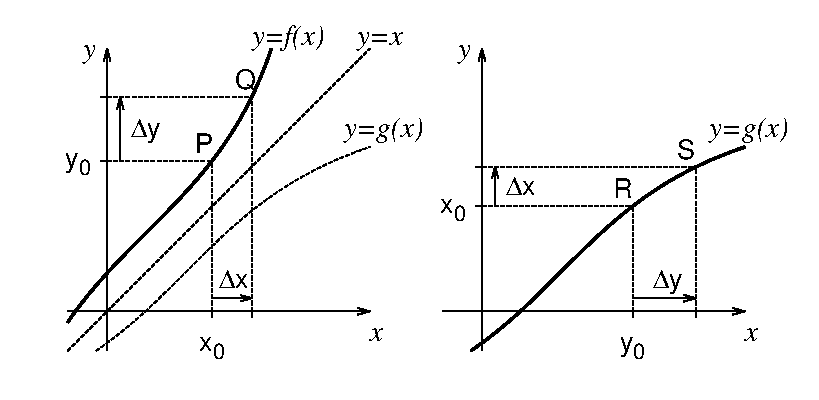
\includegraphics[width=8.5cm]{tan_atan.eps}
    \caption{関数$y=f(x)$と逆関数$y=g(x)$の微分}\label{fig:tan_atan}
\end{figure}
別の証明:
$y=f(x)$のグラフ上の2点:
\begin{eqnarray*}
\text{P: }&&(x_0, y_0)\\
\text{Q: }&&(x_0+\Delta x, y_0+\Delta y)
\end{eqnarray*}
において(\fref{fig:tan_atan}左), PとQが十分に近接していれば, 
\begin{eqnarray}
f'(x_0)\fallingdotseq\frac{\Delta y}{\Delta x}\label{eq:invdev1}
\end{eqnarray}
である。さて, $y=f(x)$のグラフを, $x$軸と$y$軸を入れ替えたら$y=g(x)$のグラフになる
のだから, 点Pや点Qの$x$座標と$y$座標を入れ替えた点
\begin{eqnarray*}
\text{R: }&&(y_0, x_0)\\
\text{S: }&&(y_0+\Delta y, x_0+\Delta x)
\end{eqnarray*}
は, 逆関数$g(x)$のグラフの上にある(\fref{fig:tan_atan}右)。RとSが十分に近接していれば, 
\begin{eqnarray}
g'(y_0)\fallingdotseq\frac{\Delta x}{\Delta y}\label{eq:invdev2}
\end{eqnarray}
である。\eref{eq:invdev1}, \eref{eq:invdev2}より, 
\begin{eqnarray}
g'(y_0)\fallingdotseq\frac{1}{\Delta y/\Delta x}\fallingdotseq\frac{1}{f'(x_0)}\label{eq:invdev3}
\end{eqnarray}
となる。$\Delta x$を0に近づける極限では右辺の$\fallingdotseq$は=になる。また, $f(x_0)=y_0$なので, 
$x_0=g(y_0)$。従って, \eref{eq:invdev3}は, 
\begin{eqnarray}
g'(y_0)=\frac{1}{f'(g(y_0))}\label{eq:invdev4}
\end{eqnarray}
となる。ここで$y_0$を改めて$x$と置きなおせば, 
\begin{eqnarray*}
g'(x)=\frac{1}{f'(g(x))}
\end{eqnarray*}
となり, \eref{eq:diff_form5}に一致する。\qed
\hv

この公\eref{eq:diff_form5}も, 一見, 複雑そうに見えるが, 以下の
ように考えれば, 実は単純である: 公\eref{eq:diff_form5}の$x$と$y$
を形式的に入れ替えれば, 
\begin{eqnarray}
g'(y)=\frac{1}{f'(g(y))}\label{eq:diff_form5c}
\end{eqnarray}
となる。ここで$x=g(y)$と置けば, $y=f(x)$だから, 
\begin{eqnarray}
&&g'(y)=\frac{dg}{dy}=\frac{dx}{dy}\label{eq:diff_form5c2}\\
&&f'(g(y))=f'(x)=\frac{df}{dx}=\frac{dy}{dx}\label{eq:diff_form5c4}
\end{eqnarray}
である。\eref{eq:diff_form5c}の左辺を\eref{eq:diff_form5c2}で, 右辺を\eref{eq:diff_form5c4}で書き換えれば, 
\begin{eqnarray}
\frac{dx}{dy}=\frac{1}{\frac{dy}{dx}}
\end{eqnarray}
と書ける。つまり, 逆関数の微分の公式は, 形式的には, 
微小量$dx$, $dy$の比の逆数をとっただけである。
そのことは, 上述のグラフを使った証明でも明らかだろう。\hv
\end{comment}

\begin{exmpl}  $f(x)=x^{1/n}$を微分してみよう。ただし$n$は1以上の整数とする。
$g(x)=x^n$とすると, $g(f(x))=x$だから, $g(x)$と$f(x)$は互いに逆関数。一方, $g'(x)=nx^{n-1}$である。
\eref{eq:diff_form5}(逆関数の微分)より, 
\begin{eqnarray}
f'(x)&=&\frac{1}{g'(f(x))}=\frac{1}{n(f(x))^{n-1}}=\frac{1}{n(x^{1/n})^{n-1}}\nonumber\\
&=&\frac{1}{nx^{(n-1)/n}}=\frac{1}{n}x^{-(n-1)/n}\nonumber\\
&=&\frac{1}{n}x^{(1-n)/n}=\frac{1}{n}x^{(1/n)-1}\label{eq:xpowfrc}
\end{eqnarray}
(例おわり)\end{exmpl}

\eref{eq:xpowfrc}は, \eref{eq:diff_x}で$n$を$1/n$と置き換えたものに一致する。
これで, \eref{eq:diff_x}は, 定数$n$が正の整数の逆数のときも成り立つことがわかった。

\eref{eq:diff_x}, \eref{eq:xpowminusn3}, \eref{eq:xpowfrc}からわかったように, 
定数$\alpha$が正の整数または負の整数または正の整数の逆数のとき, 
\begin{eqnarray}(x^{\alpha})'=\alpha x^{\alpha-1}\end{eqnarray}
が成り立つ。そのことと合成関数の微分の公式を使えば, $\alpha$が負の整数の逆数
のときや, 0以外の有理数(整数どうしの比であらわされる数)のときもこれが成り立つこと
が証明できる。実数は有理数の極限としてあらわされるので
\footnote{このあたりは高度な数学になるので, 詳細はわからなくてもよい。}, 有理数で成り立てば, 実数でも成り立つ。
従って, 以下の公式が成り立つ:\hv

\begin{itembox}{微分の公式6: べき関数の微分}
定数$\alpha$が0以外の実数であれば, 
\begin{eqnarray}
(x^{\alpha})'=\alpha x^{\alpha-1}\label{eq:diff_form6}
\end{eqnarray}
\end{itembox}

\begin{exmpl} もういちど関数$f(x)=1/x$を微分してみよう。$1/x=x^{-1}$だから, \eref{eq:diff_form6}
で$\alpha=-1$とすれば, 
\begin{eqnarray}
f'(x)=(x^{-1})'=-1\cdot x^{-2}=-\frac{1}{x^2}
\end{eqnarray}
これは式(\ref{eq:dif_recipr})と一致する。つじつまがあっている。(例おわり)\end{exmpl}

\begin{exmpl} $\sqrt{x}$を微分してみよう。
\begin{eqnarray}
(\sqrt{x})'=(x^{1/2})'=\frac{1}{2}\,x^{1/2-1}=\frac{1}{2}x^{-1/2}=\frac{1}{2\sqrt{x}}\nonumber\\
\end{eqnarray}
(例おわり)\end{exmpl}

%----------
\begin{q}\label{q:diff_pow} 公式6を使って, 以下の関数を微分せよ。
\begin{edaenumerate}<4>
\item \begin{eqnarray*}\frac{1}{x}\,\,\,\,\,\,\,\,\end{eqnarray*}
\item \begin{eqnarray*}\frac{1}{\sqrt{x}}\,\,\,\,\,\,\,\,\end{eqnarray*}
\item \begin{eqnarray*}x^{2/3}\,\,\,\,\,\,\,\,\end{eqnarray*}
\item \begin{eqnarray*}x^{-5}\,\,\,\,\,\,\,\,\end{eqnarray*}
\end{edaenumerate}\end{q}
\mv

%----------
\begin{q}\label{q:diff_theories1_5} 微分の公式1〜5を証明せよ。\end{q}
\mv

微分の計算は, とにかくたくさん練習して, 規則性を体に染み込ませよう。
微分の定義はとても大切だけど, 実際の関数を手計算で微分するときは, 
微分の定義よりもむしろ, これまで見てきたようないろいろな公式を
機械的に適用するのだ。\hv

\begin{exmpl}\label{exmpl:diff_sqrtx2p1} $\sqrt{x^2+1}$を微分してみよう。$g(x)=\sqrt{x}$と
$f(x)=x^2+1$の合成関数$g(f(x))$とみなして, 
\begin{eqnarray}
(\sqrt{x^2+1})'&=&\frac{1}{2\sqrt{x^2+1}}\times(x^2+1)'\nonumber\\
                &=&\frac{2x}{2\sqrt{x^2+1}}=\frac{x}{\sqrt{x^2+1}}\label{eq:exmpl_diff_23}
\end{eqnarray}
(例おわり)\end{exmpl}

\begin{exmpl} $x\sqrt{x^2+1}$を微分してみよう。
\begin{eqnarray}
(x\sqrt{x^2+1})'&=&x'\sqrt{x^2+1}+x(\sqrt{x^2+1})'\nonumber\\
                &=&\sqrt{x^2+1}+x\times\frac{x}{\sqrt{x^2+1}}\nonumber\\
                &=&\sqrt{x^2+1}+\frac{x^2}{\sqrt{x^2+1}}
\end{eqnarray}
最初の変形では積の微分(公式3)を使った($x$と$\sqrt{x^2+1}$の積)。それ以降は\eref{eq:exmpl_diff_23}の
結果を使った。(例おわり)\end{exmpl}
\mv

\begin{freqmiss}{\small\textgt{微分記号を省略し, 微分する前の関数と微分した
後の関数をイコールで結んでしまう。例えば, $(x^2+x)'=2x+1$と
書くべきところを, $x^2+x=2x+1$と書いてしまう。}}\end{freqmiss}
\mv

%----------
\begin{q}\label{q:diff_func8} 微分の公式を駆使して, 以下の関数を微分せよ:
\begin{edaenumerate}<3>
\item \begin{eqnarray*}\sqrt{2x+3}\,\,\,\,\,\,\,\,\,\,\,\,\,\,\,\end{eqnarray*}
\item \begin{eqnarray*}\sqrt{1-x^2}\,\,\,\,\,\,\,\,\,\,\,\,\,\,\,\end{eqnarray*}
\item \begin{eqnarray*}x^2\sqrt{1+x^2}\,\,\,\,\,\,\,\,\,\,\,\,\,\,\,\end{eqnarray*}
\item \begin{eqnarray*}\frac{1}{\sqrt{1+x^2}}\,\,\,\,\,\,\,\,\,\,\,\,\,\,\,\end{eqnarray*}
\item \begin{eqnarray*}\frac{1}{1+\sqrt{x}}\,\,\,\,\,\,\,\,\,\,\,\,\,\,\,\end{eqnarray*}
\item \begin{eqnarray*}\sqrt{1+\frac{1}{x}}\,\,\,\,\,\,\,\,\,\,\,\,\,\,\,\end{eqnarray*}
\item \begin{eqnarray*}\frac{x-1}{x+1}\,\,\,\,\,\,\,\,\,\,\,\,\,\,\,\end{eqnarray*}
\item \begin{eqnarray*}\frac{1}{1+\frac{1}{x}}\,\,\,\,\,\,\,\,\,\,\,\,\,\,\,\end{eqnarray*}
\end{edaenumerate}\end{q}
\vv



\section{線型近似}

\eref{eq:define_dif_Delta}で述べたように, 関数$f(x)$の, $x=x_0$における微分係数$f'(x_0)$は,
\begin{equation}
f(x_0+\Delta x) \fallingdotseq f(x_0) + f'(x_0) \Delta x
\end{equation}
を満たす。$\Delta x$が0に近ければ近いほど, 近似等号"$\fallingdotseq$"は等号"$=$"に
近づくのだが, たとえ有限小の$\Delta x$についても$f(x_0+\Delta x)$を, 
この右辺の式で置き換え, ざっくりと近似することがよくある。
これを関数の\underline{線型近似} \index{せんけいきんじ@線型近似} (一次近似
\index{いちじきんじ@一次近似})という。要するに, 関数を一次式で近似するのだ。
グラフで言えば, 曲線を, その接線で近似するのだ。

\begin{faq}{\small\textgt{それって, 数値微分の考え方に似てません?}
... そうです。というより, 数値微分は, 線型近似の考え方を使っているのです。}\end{faq}

線型近似は誤差が出てしまうが, 多少の誤差はOKという状況で式や
計算を単純化したいときにとても便利である。

特に, $x_0=0$とし, 0に近い範囲でしか$x$を考えないという前提で, $\Delta x$を$x$と置き換えることで, 
\begin{eqnarray}
f(x) \fallingdotseq f(0)+f'(0)x\label{eq:linear_approx00}
\end{eqnarray}
となる。実用上は, このタイプの近似式が, よく使われる。
では実際に線型近似をやってみよう。\mv

\begin{exmpl} $\,\,\,\,\,f(x)=\sqrt{1+x}$ を線型近似する:\\
$f'(x)=1/(2\sqrt{1+x})$なので, $f(0)=1, f'(0)=1/2$。これを\eref{eq:linear_approx00}
に入れると, $x=0$付近で
\begin{eqnarray}
\sqrt{1+x}\fallingdotseq 1+\frac{x}{2}\label{eq:linear_approx01}
\end{eqnarray}
となる。試しに, 実際にいくつかの値を計算してみよう。

$\sqrt{1.1}=1.04880...$だが, \eref{eq:linear_approx01}より, 
$\sqrt{1.1}=\sqrt{1+0.1}\fallingdotseq1+0.1/2=1.05$。

$\sqrt{1.01}=1.004987...$だが, \eref{eq:linear_approx01}より, 
$\sqrt{1.01}=\sqrt{1+0.01}\fallingdotseq1+0.01/2=1.005$。
(例おわり)\end{exmpl}
\mv

\begin{q}\label{q:univ_lin_approx0} $x=0$付近で, 以下の式が成り立つことを示せ(ただし$a$は任意の実数)。
\begin{eqnarray}
(1+x)^a\fallingdotseq1+ax\label{eq:linear_approx02}
\end{eqnarray}\end{q}

\eref{eq:linear_approx02}の形の線型近似はとてもよく使われる。

\begin{q}\label{q:univ_lin_approx2} 以下の関数を, $x=0$付近で線型近似せよ:
\begin{edaenumerate}<3>
\item $1/(1+x)$
\item $1/(1-x)$
\item $1/\sqrt {1+x}$
\end{edaenumerate}\end{q}
\mv

\eref{eq:linear_approx02}を利用すると, 多くの計算を(近似的にだが)簡単にできる。\mv

\begin{exmpl} $\,\,\,\,\,(1.01)^{10}$の近似値を求めよう。
これがもし$1^{10}$なら楽である。そこで, $1.01=1+0.01$というふうに考える: 
$(1+0.01)^{10} \fallingdotseq 1+10\times0.01 = 1.1$\\
正確には$(1.01)^{10}=1.1046\cdots$であり, 有効数字3桁まで合っている。
\end{exmpl}

\begin{exmpl} $\,\,\,\,\,\sqrt{26}$の近似値を求めよう。2乗して
26に近い数は何かな?と考えると, $5^2=25$である。そこで, 
$26=25+1$と考える。
\begin{eqnarray*}
\sqrt{26}&&=\sqrt{25+1}=\sqrt{25\Bigl(1+\frac{1}{25}\Bigr)}=5\sqrt{1+\frac{1}{25}}\\
&&\fallingdotseq5\Bigl(1+\frac{1}{50}\Bigr)=5.1
\end{eqnarray*}
正確には$\sqrt{26}=5.0990\cdots$であり, 有効数字3桁まで合っている(4桁目を四捨五入
すると一致する)。この式展開で, 25を先に$\sqrt{\quad}$の外に追い出し, $\sqrt{\quad}$の
中を$1+1/25$の形にしたところがコツなのだ。$1/25$は0にそこそこ近いので, 
\eref{eq:linear_approx02}が使えたのだ。このように, まずざっくり簡単な
近似値(この場合は5)を勘で見つけることが大事。それをもとに, 線型近似で精度を
上げるのだ。(例おわり)\end{exmpl}
\mv

\begin{q}\label{q:univ_lin_approx4} 線型近似を利用して, 以下の値を近似的に求めよ(電卓を使わないで筆算で。できれば暗算で!):
\begin{enumerate}
\item $(0.99)^{10}$ (正確には$0.9043\cdots$となる)
\item $10^{1/3}$ (正確には$2.1544\cdots$となる)
\end{enumerate}\end{q}
\mv


\section{高階導関数}

ところで, 関数$f(x)$を, 2回続けて微分することを考えよう。それを, \underline{2階微分}とか
\underline{2階導関数} (「回」ではなく「階」という字を使う)と呼び, $f''(x)$と書く(定義)。
2階導関数$f''(x)$は, \eref{eq:define_dif45}の書き方で書けば, 
\begin{eqnarray}
\frac{d}{dx}\Bigl(\frac{d}{dx}f(x)\Bigr)
\end{eqnarray}
とも書けるので, 形式的に縮めて, 
\begin{eqnarray*}
\frac{d^2}{dx^2}f(x)\quad\text{とか,}\quad 
\frac{d^2f}{dx^2}(x)\quad\text{とか,}\quad 
\frac{d^2f}{dx^2}
\end{eqnarray*}
と書くこともある。分母と分子で「2乗」のつく位置が異なることに注意。

これと同様に考えて, 「3階導関数」「4階導関数」...「$n$階導関数」など($n$は1以上の整数)も
考えることができ, それらはまとめて\underline{高階導関数} \index{こうかいどうかんすう@高階導関数}と呼び, 
\begin{eqnarray}
&&f^{(n)}(x)\label{eq:diff_mult_def1}\\
&&\frac{d^n}{dx^n}f(x)\label{eq:diff_mult_def2}\\
&&\frac{d^nf}{dx^n}(x)\label{eq:diff_mult_def3}\\
&&\frac{d^nf}{dx^n}\label{eq:diff_mult_def4}
\end{eqnarray}
などと書く。独立変数$x$やその値が文脈上, 明らかであれば, \eref{eq:diff_mult_def4}のように, 
$(x)$は省略してもかまわない。\eref{eq:diff_mult_def1}については, $n$個の
ダッシュ「$'$」を書きたいところだが, $f''''''(x)$とか書くのは格好が
悪いので, 3階以上になったら, $(3)$とか$(n)$というふうに書く。\hv

%----------
\begin{q}\label{q:diff_func9} 以下の関数について, $f'(x)$, $f''(x)$, $f^{(3)}(x)$をそれぞれ求めよ。
\begin{edaenumerate}
\item \begin{eqnarray*}f(x)=x^5+2x^3\,\,\,\,\,\,\,\,\,\,\end{eqnarray*}
\item \begin{eqnarray*}f(x)=\frac{1}{1-x}\,\,\,\,\,\,\,\,\,\,\end{eqnarray*}
\end{edaenumerate}\end{q} 
\mv

\begin{faq}{\small\textgt{$d^2x/dt^2$の,$dt^2$や
$d^2x$はどういう状態?} ... 
既に述べたように, $dt^2$は$dt$かける$dt$です。
$d^2x$は, $t$が2段階で変化するときの「$x$の変化の変化」
と思えばよろしい。つまり, $t$が$t+dt$に変化した時の$dx$と, 
$t$が$t+dt$から$t+2dt$に変化した時の$dx$との差(後者引く前者)
が$d^2x$です。丁寧に書くと, $d(dx)$です。$dx$自体が微小量
だから, 微小量どうしの差はすごく小さい微小量になるという
ことが直感できるでしょう。$dt^2$や$d^2x$を「2次の微小量」
と言います。2次の微小量は$dt$や$dx$という1次の微小量
よりはるかに小さいので, 普通, 無視します(0とみなします)
が, この場合は, 2次の微小量どうしの比を考えているので, 
無視できないのです。

ところで, 高校で, $dx/dt$はそれ全体でひとつの記号
であり, 「$dx$わる$dt$」ではない, と習った人も
いるでしょう。厳密な数学はそのような立場です。しかし, 
生物資源学類が関わる多くの応用的な学問では, 
$dx/dt$を「$dx$わる$dt$」と考えてほとんど差し支えないし, 
その方が理解も応用もしやすいので, この授業ではその立場を
とります。}\end{faq}


\section{微分ができない場合}

ここまで読んで, 君は, どんな関数でも微分できるような気がしているかも
しれない。でも, 世の中には微分ができない(導関数や微分係数が存在しない)場合
もたくさんある。

\begin{exmpl}\label{ex:Nodif_1/x} 以下の関数
\begin{eqnarray}f(x)=\frac{1}{x}\end{eqnarray}
は, $x=0$以外では微分できて, 導関数は$f'(x)=-1/x^2$だ。では$x=0$では微分
できるだろうか? そもそも微分の定義である\eref{eq:define_dif}や
\eref{eq:define_dif2}に戻ると, 微分を考えるには$f(x_0)$の値が必要だ。
今は$x_0=0$を考えているので$f(0)$が必要。でもこの関数に$f(0)$は
存在しない(0での割り算は禁じ手である。$1/0=\infty$だと思っている
人もいるだろうが, $\infty$というのは数ではないのだ)。
なので, この関数は$x=0$では微分できない。(例おわり)
\end{exmpl}

この例\ref{ex:Nodif_1/x}では, 微分したい位置でそもそも関数の値が定まって
いなかった。そういう場合, 微分はできない。分数で表される関数で分母が0
になるときにこのような状況になることが多い。

\begin{exmpl}\label{ex:Nodif_|x|} 以下の関数
\begin{eqnarray}f(x)=|x|\label{eq:f(x)=|x|}\end{eqnarray}
の微分を考えよう。これは, 
\begin{eqnarray*}
f(x)=\begin{cases}
-x\,\,\,\,\,\,\,\,\,\,(x<0\text{のとき})\\
x\,\,\,\,\,\,\,\,\,\,\,\,\,(0\leq x\text{のとき})
\end{cases}\end{eqnarray*}
ということだ。従って, 導関数は
\begin{eqnarray}
f'(x)=\begin{cases}
-1\,\,\,\,\,\,\,\,\,\,(x<0\text{のとき})\\
1\,\,\,\,\,\,\,\,\,\,\,\,\,(0\leq x\text{のとき})
\end{cases}\label{eq:|x|'2}\end{eqnarray}
だと思うかもしれない。これはおおむね正しいが, \textgt{$x=0$のところで間違っているのだ}。
微分の定義である\eref{eq:define_dif}に戻ってみよう(\eref{eq:define_dif2}に戻っても
結論は同じ)。$x_0=0$とすれば, \eref{eq:define_dif}は
\begin{eqnarray}f(0+dx) = f(0)+f'(0)dx\label{eq:|x|'3}\end{eqnarray}
となる。ここで\eref{eq:f(x)=|x|}より, $f(0)=0$だから, \eref{eq:|x|'3}は
\begin{eqnarray}f(dx) = f'(0)dx\label{eq:|x|'4}\end{eqnarray}
となる。もし, \eref{eq:|x|'2}が正しければ, $f'(0)=1$となり, 従って\eref{eq:|x|'4}は
\begin{eqnarray}f(dx) = dx\label{eq:|x|'5}\end{eqnarray}
となるはず。ところが$dx$は0に近い任意の微小量なので, $dx<0$となる場合もあるだろう。
その場合, \eref{eq:|x|'5}から, $f(dx)<0$となる。ところが\eref{eq:f(x)=|x|}より, 
この関数は決して負の値をとることはあり得ない。従って矛盾する。従って, \eref{eq:|x|'2}は
$x=0$で正しくない\footnote{このような論法を「背理法」という。第\ref{chapt_logic}章参照。}。
同様に考えれば, $f'(0)$をどのような値にしても矛盾が生じることがわかるだろう。
従って, $f'(0)$は存在しない, すなわちこの関数は$x=0$では微分できない。(例おわり)
\end{exmpl}

この例\ref{ex:Nodif_|x|}で出てきた\eref{eq:f(x)=|x|}のグラフを図\ref{fig:abs_x}に示す。
微分したい位置($x=0$)で, グラフが尖っている。詳細は省くが, 一般に, グラフが尖っている
箇所では, 関数は微分不可能である。式に絶対値記号が入っていて, 絶対値記号の内側が0
になるときにこういう状況になることが多い
\footnote{ただしそうでないときもある。$f(x)=|x|^3$は$x=0$で絶対値記号内が0になるが, 
$x=0$で微分可能である。}。
\begin{figure}[h]
    \centering
    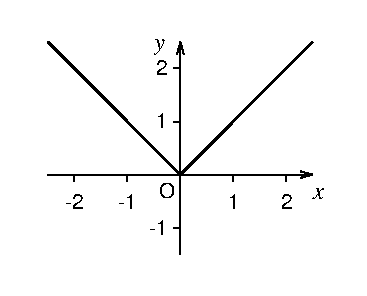
\includegraphics[width=5cm]{abs_x.eps}
    \caption{関数$y=|x|$のグラフ。$x=0$で微分不可能(尖っている)。}\label{fig:abs_x}
\end{figure}

\begin{exmpl}\label{ex:Nodif_01} 以下の関数
\begin{eqnarray}
f(x)=\begin{cases}
0\,\,\,\,\,\,\,\,\,\,(x<0\text{のとき})\\
1\,\,\,\,\,\,\,\,\,\,\,(0\leq x\text{のとき})
\end{cases}\label{eq:01'1}\end{eqnarray}
の微分を考えよう。定数関数の微分は0だから, 
\begin{eqnarray}
f'(x)=\begin{cases}
0\,\,\,\,\,\,\,\,\,\,(x<0\text{のとき})\\
0\,\,\,\,\,\,\,\,\,\,\,(0\leq x\text{のとき})
\end{cases}\label{eq:01'2}\end{eqnarray}
つまり, $f'(x)=0$のように思うかもしれない。これも, おおむね正しいが, 
\textgt{$x=0$のところで間違っているのだ!} 再び微分の定義である\eref{eq:define_dif}
に戻って考えてみよう。$x_0=0$, $f(x_0)=f(0)=1$とすれば, \eref{eq:define_dif}は
\begin{eqnarray}f(dx) = 1+f'(0)dx\label{eq:01'4}\end{eqnarray}
となる。もし, \eref{eq:01'2}が正しければ, $f'(0)=0$となり, 従って\eref{eq:01'4}は
\begin{eqnarray}f(dx) = 1\label{eq:01'5}\end{eqnarray}
となるはずだ。ところが$dx$は0に近い任意の微小量なので, $dx<0$となる場合もあるだろう。
その場合, \eref{eq:01'1}より, $f(dx)=0$となるはずで, これは\eref{eq:01'5}
に矛盾する。従って, $f'(0)=0$は$x=0$では成り立たない。実は, $f'(0)$にどのような
値を与えても, これらのつじつまを合わせることはできないのだ。(例おわり)
\end{exmpl}

\eref{eq:01'1}のグラフを図\ref{fig:step_func01}に示す。$x=0$でグラフがつながって
いない。詳細は省くが, 一般に, グラフがつながっていない\footnote{グラフがつながっていない, 
ということはどういうことかを, 数学的に定義するのは, 実は簡単なことでは無い。}
ようなところでは, 関数は微分できない。

\begin{figure}[h]
    \centering
    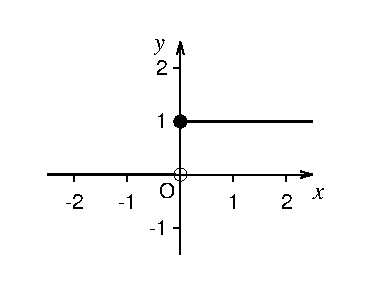
\includegraphics[width=5cm]{step_func01.eps}
    \caption{\eref{eq:01'1}の$y=f(x)$のグラフ。$x=0$で微分不可能(つながっていない)。}\label{fig:step_func01}
\end{figure}



\begin{exmpl}\label{ex:Nodif_xpow1/3} 以下の関数
\begin{eqnarray*}
f(x)=x^{1/3}
\end{eqnarray*}
の微分を考えよう。機械的に導関数を計算すると, 
\begin{eqnarray}f'(x)=\frac{1}{3x^{2/3}}\label{eq:xpow1/3'}\end{eqnarray}
となる。これは正しいのだが, この式では$x=0$での値が定まらない。つまり, この関数
は$f'(0)$を持たない。(例おわり)
\end{exmpl}

この例\ref{ex:Nodif_xpow1/3}では, 微分したい位置($x=0$)で, 関数の値は定まるが
導関数の値が定まらない($\infty$になってしまう)。グラフ(図\ref{fig:xpow1_3})
を見ると, $x=0$での傾きが無限大(接線が$x$軸に垂直)になりそうだ。詳細は省くが, 
グラフが垂直に立つようなところでは, 関数は微分できない。

\begin{figure}[h]
    \centering
    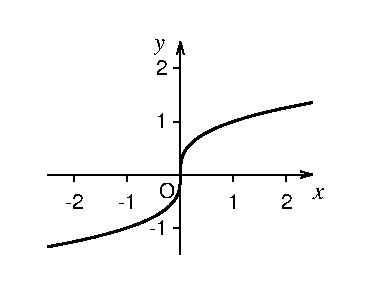
\includegraphics[width=5cm]{xpow1_3.eps}
    \caption{$y=x^{1/3}$のグラフ。$x=0$で微分不可能(傾きが$\infty$になる)。}\label{fig:xpow1_3}
\end{figure}

では, どのような場合なら微分可能なのだろうか? 数学的には, \eref{eq:define_dif}や
\eref{eq:define_dif2}によって$f'$が一意的に定義できる場合, 微分可能である。とは
いえ, いちいち\eref{eq:define_dif}や\eref{eq:define_dif2}に戻るのは大変だ。
さしあたって実用的には, 場合分けや絶対値記号が無く, 導関数の式を導くことができ, 
微分したい位置の$x$の値をもとの関数と導関数の両方に代入してそれぞれ値が定まる
ようならば, ほとんどの場合で微分できると思ってよい。
\vv




\section{速度・加速度} \label{secvelocity_and_acceleration}

さて, 微分は物理学で非常によく使われる。そもそも, 微分という概念は物理学上の必要
に迫られて発明されたのだ(それが今では, 化学・生物学・経済学・統計学等の広範な
学問に不可欠な道具になっている)。物理学で最初に出てくる微分は, 速度や加速度という考え方
である。それを学ぶために, まず準備として, いくつかの言葉を確認しておこう:
 
いま, $x$軸上を移動する点Pがあるとする。時刻$t$のときのPの位置($x$座標)を$x(t)$とする。
ある時刻$t_0$ではPは$x(t_0)$にあり, 別の時刻$t_1$ではPは$x(t_1)$にある。

2つの時刻の差, すなわち$t_1-t_0$を「時刻差」という\footnote{実際は「時刻差」という
言葉はめったに使わないが, ここでは時刻や時間と区別するために導入する。}。
$t_1>t_0$なら時刻差$t_1-t_0$は正の値をとるし, $t_1<t_0$なら時刻差$t_1-t_0$は負の値をとる。
時刻差$t_1-t_0$の絶対値, すなわち$|t_1-t_0|$を「時間」という。時間は常に0以上の値をとる。

2つの位置の差を変位(displacement)\index{へんい@変位}という。
今の場合, $x(t_1)-x(t_0)$が変位である。$x(t_1)>x(t_0)$なら変位は
正の値をとるし, $x(t_1)<x(t_0)$なら変位は負の値をとる。変位の絶対値
を「距離」(distance)\index{きょり@距離}という。今の場合, $|x(t_1)-x(t_0)|$が距離である。
当然ながら, 距離は常に0以上の値をとる。

まとめると, 
\begin{itemize}
\item $t$ ... 時刻
\item $t_1-t_0$ ... 時刻差 (時刻の差)
\item $|t_1-t_0|$ ... 時間 (時刻差の絶対値)
\item $x(t)$ ... 位置
\item $x(t_1)-x(t_0)$ ... 変位 (位置の差)
\item $|x(t_1)-x(t_0)|$ ... 距離 (変位の絶対値)
\end{itemize}
である。

さて, 「時刻$t_0$から$t_1$の間のPの平均速度$\overline{v}$」を, 次式で定義する:
\begin{eqnarray}\overline{v} :=\frac{x(t_1)-x(t_0)}{t_1-t_0}\label{eq:veloc_mean_def}\end{eqnarray}
すなわち, 平均速度とは変位を時刻差で割ったものだ。
\eref{eq:veloc_mean_def}で, もし時刻差が正で変位が負ならば, 
平均速度は負の値になる。このとき, Pは$x$軸の負の向きに進んでいる。
このように, 平均速度の正負は移動の向きを表す。

さて, \eref{eq:veloc_mean_def}で定義した「平均速度」は, 
時刻$t_0$と時刻$t_1$の間で物体の運動が勢いを増したり減らしたり, 
刻々と変化するような様子を表現できない。そのような細かな変化も表現する
には, 時刻$t_0$と時刻$t_1$の間をできるだけ短くして表現しなければならない。そこで, 
\eref{eq:veloc_mean_def}の$t_1$が, 限りなく$t_0$に近い場合(極限)
を考えよう。そのような極限は, 次式のようになる:
\begin{eqnarray}v(t_0):=\lim_{t_1\rightarrow t_0}\frac{x(t_1)-x(t_0)}{t_1-t_0}\label{eq:veloc_def0}\end{eqnarray}
あるいは$t_1-t_0=\Delta t$と書いて, 
\begin{eqnarray}v(t_0):=\lim_{\Delta t\rightarrow 0}\frac{x(t_0+\Delta t)-x(t_0)}{\Delta t}\label{eq:veloc_def1}\end{eqnarray}
と書く。この式を\eref{eq:define_dif2}と比べてみるとわかるように, これは
$x(t)$という関数の, $t=t_0$での微分係数である。これを「時刻$t_0$で
の\underline{速度} \index{そくど@速度}(velocity)」と言う。要するに
速度とは位置を時刻で微分したものである(定義)。このように定義した速度を, 
上述の「平均速度」と区別するためにわざわざ「瞬間の速度」と言うこともある。

時刻$t$における速度$v(t)$は, 定義より, $x'(t)$と書ける。物理学では, 
$x'(t)$のことを$\dot{x}$と表すこともある(上付きのドットが「時刻による微分」
を表すのだ)。つまり,
\begin{eqnarray}v(t)=\frac{dx}{dt}=x'(t)=\dot{x}\label{eq:veloc_def2}\end{eqnarray}
である。このように, 同じことをいろんな記法で表すことがある。

さて, 平均速度の正負が運動の方向を表したように, (瞬間の)速度にも正負が
あり, それは運動の方向を表す。

ここで, 速度の絶対値のことを\underline{速さ} (speed)と呼ぶ(定義)。
例えば\eref{eq:veloc_mean_def}の左辺と右辺のそれぞれ絶対値をとると, 
\begin{eqnarray}|\overline{v}|=\frac{|x(t_1)-x(t_0)|}{|t_1-t_0|}\label{eq:veloc_mean_def_abs}\end{eqnarray}
となる。これを平均速さという。
右辺の$|x(t_1)-x(t_0)|$は距離, $|t_1-t_0|$は時間なので, 
\eref{eq:veloc_mean_def_abs}は, \\
  「平均速さ=距離÷時間」\\
となる。ところが小学校では\\
  「速さ=距離÷時間」\\
と習った。つまり, 小学校で習った
「速さ」は, 正確に言うと「平均速さ」だったのだ。 
\eref{eq:veloc_mean_def_abs}で$t_1$を$t_0$に近づける極限は, 
(瞬間の)速度の絶対値であり, それを(瞬間の)速さという。

「速さ」は「速度」の大きさ(絶対値)なので, 必ず
0以上の値である。負の値をとることはない。つまり速さには
「向き」の概念が無い。逆に言えば, 速さと向きをセット
にした概念が速度である。\hv

\begin{freqmiss}{\small\textgt{
「速度は\textgt{距離}を時刻で微分したものである」
「速度は位置を微分したものである」などと言ってしまう} ... 
前者は, 距離ではなくて位置。後者は間違いではありませんが, どういう量
について(この場合は時刻)微分するのかもきちんと言わねばなりません。}
\end{freqmiss}

\begin{q}\label{q:diff_def}  
\begin{enumerate}
\item 平均速度と速度はどう違うか?
\item 速度と速さはどう違うか?
\item 速度と速さはぞれぞれどのような英語単語で表現されるか?
\item 「速度とは距離を時刻で微分したものだ」という発言はどこが間違っているか?
\item 「速度とは位置を微分したものだ」という発言はどこが間違っているか?
\end{enumerate}\end{q}
\hv

\eref{eq:define_dif}, \eref{eq:veloc_def2}より, 次式のようにも書ける:
\begin{eqnarray}
x(t+dt) = x(t) + v(t)dt\label{eq:xtdtxtvtdt}
\end{eqnarray}
ここで$dt$は微小な時刻差である。この\eref{eq:xtdtxtvtdt}によれば, 
$dt$だけ時刻が変化したときの位置(つまり$x(t+dt)$)は, 現在の位置(つまり$x(t)$)
から, $v(t)dt$だけ変化する(速度も, 時刻とともに変わるかもしれないが, 
$t$と$t+dt$の間では,ほとんど一定とみなすことができるだろう。というより
むしろ, 速度がほぼ一定とみなせるくらいに短い$dt$を考える)。つまり, 時刻差
が微小な場合は, 変位は速度と時刻差の積に等しい。それは, \eref{eq:xtdtxtvtdt}を
\begin{eqnarray}
x(t+dt)-x(t) = v(t)dt\label{eq:xtdtxtvtdt2}
\end{eqnarray}
と変形すれば, より明らかだろう。
ここで, \eref{eq:xtdtxtvtdt2}について両辺の絶対値をとると, 
\begin{eqnarray}
|x(t+dt)-x(t)| = |v(t)||dt|\label{eq:xtdtxtvtdt3}
\end{eqnarray}
となる。左辺は距離, 右辺は速さと時間の積である(速度の絶対値を「速さ」
というのだから, $|v(t)|$が「速さ」である)。これは, 小学校で習った, 
\begin{eqnarray}\text{距離}=\text{速さ}\times\text{時間}\end{eqnarray}
と整合的である。\hv

速度を時刻で微分したものを\underline{加速度} (acceleration)\index{かそくど@加速度}と言う(定義)。
すなわち, 時刻$t$における加速度$a(t)$とは, 
\begin{eqnarray}a(t)=v'(t)\label{eq:ac_def2}\end{eqnarray}
である。\eref{eq:define_dif}を
使って\eref{eq:ac_def2}を書き換えれば, 
\begin{eqnarray}v(t+dt) &=& v(t) + a(t)dt\label{eq:vtdtvtatdt}
\end{eqnarray}
となる。また, \eref{eq:veloc_def2}を使えば, \eref{eq:ac_def2}は, 
\begin{eqnarray}a(t)=v'(t)=x''(t)\label{eq:ac_def3}\end{eqnarray}
となる。すなわち, 加速度は位置を時刻で二階微分したものでもある。

\begin{faq}{\small\textgt{物理で, 速度の定義は「単位時間あたりの変位」
と習ったのですが。}... それでもいいですよ。それを数学的に言えば, 
位置を時刻で微分したもの, となります。同様に, 加速度を「単位時間あたりの
速度変化」と定義しても構いません。一般に, 「単位...あたりの---の変化」
とは, 数学的には「---を...で微分したもの」です。}\end{faq}\mv

%-----------------
\begin{q}\label{q:diff_velocac} 点Pが直線上を運動している。
時刻$t$のときPの位置(ある基準点から測った距離)を$x$とすると, 
次式のように書けるとする($a, b, c$は$t$によらない適当な定数):
\begin{eqnarray}
x=a\,t^2+b\,t+c\label{eq:diff_velocac03}
\end{eqnarray}
\begin{enumerate}
\item 時刻$t$におけるPの速度は? 
\item 時刻$t$におけるPの加速度は? 
\end{enumerate}
\end{q}
\vspace{0.3cm}

さて, 物理量を物理量で微分すると, 次元が変わることに注意しよう。
例えば, 位置の次元は「長さ」だが, 位置を時刻で微分して速度にすると, 
その次元は「長さ/時間」
となる。なぜ次元が変わるのだろう? それは\eref{eq:veloc_def1}を見れば
わかる。分母に$\Delta t$がある。つまり, 時刻で微分するときは, 
「時間で割っている」のだ。一般に, 量$p$を量$q$で微分して得られる量の
次元は「$p$の次元」/「$q$の次元」になる。従って, 速度をさらに時刻で
微分すると, 次元は「長さ/時間$^2$」になる。\hv

\begin{q}\label{q:diff_velocac1} \eref{eq:diff_velocac03}
において, $a, b, c$はそれぞれどのような次元を持つべきか?\end{q}

\begin{q}\label{q:diff_velocac2} 上の問\ref{q:diff_velocac}
において, $a=4.9$~m~s$^{-2}$, $b=1$~m~s$^{-1}$, $c=3$~mの
とき, $t=10$~sでの, 位置, 速度, 加速度をそれぞれ求めよ。
\end{q}


\section{ベクトルの微分}

前節で学んだことを, 2次元平面や3次元空間に拡張しよう。それには, 
ベクトルが必要になる。

空間の中を, 時刻とともに移動する点を考える。時刻$t$のときの
点の位置を, 位置ベクトル${\bf r}(t)$で表そう。これは時刻と
共に次第に変化していくベクトルである。この位置ベクトルを, 
${\bf r}(t)=(x(t), y(t), z(t))$というふうに座標で表すと, その
各成分は時刻$t$の関数である。各成分の微分を考えると, 
\eref{eq:define_dif}より, 
\begin{eqnarray}\begin{cases}
x(t+dt)=x(t)+x'(t)dt\\
y(t+dt)=y(t)+y'(t)dt\\
z(t+dt)=z(t)+z'(t)dt
\end{cases}\end{eqnarray}
である。ここで, 
\begin{eqnarray}
{\bf r}'(t)=(x'(t), y'(t), z'(t))
\end{eqnarray}
と定義すれば, 上の3つの式は, まとめて
\begin{eqnarray}
{\bf r}(t+dt)={\bf r}(t)+{\bf r}'(t)\,dt\label{eq:diff_rt}
\end{eqnarray}
と書ける。これは\eref{eq:define_dif}によく似ている。これが
微分の「ベクトル版」である。ベクトルを値にとるような
関数${\bf r}(t)$は, \eref{eq:diff_rt}によって, その微分係数${\bf r}'(t)$
が定義されるのだ。

\begin{faq}{\small\textgt{ちょっと混乱してきました。微分って, グラフの
接線の傾きですよね。ベクトルを値にとるような関数${\bf r}(t)$の「グラフ」とか, 
その「接線の傾き」はどうイメージすればいいのですか?} ... そういうことになる
から, 「微分はグラフの接線の傾き」というイメージを持ち過ぎないように, 
と言ったのです! この場合は「グラフの接線の傾き」はイメージできないし, する
必要もありません。微分のイメージは, 「微小量どうしの比例関係の比例係数」
です。\eref{eq:diff_rt}で言えば, ${\bf r}(t+dt)-{\bf r}(t)$を
微小なベクトル量$d{\bf r}$とすれば, $d{\bf r}={\bf r}'(t)\,dt$となって
おり, $d{\bf r}$と$dt$が比例してるでしょ? その比例係数${\bf r}'(t)$が
${\bf r}(t)$の微分なのです。}\end{faq}

さて, 位置ベクトル${\bf r}(t)$を時刻$t$で微分したものを, 
「速度ベクトル」\index{そくどべくとる@速度ベクトル}あるいは単に「速度」と言う(定義)。
速度は, その英語"velocity"の頭文字をとって, ${\bf v}(t)$と表すことが多い。すなわち, 
\begin{eqnarray}
{\bf v}(t):={\bf r}'(t)=(x'(t), y'(t), z'(t))
\end{eqnarray}
である。この記号を使うと, \eref{eq:diff_rt}は次式になる:
\begin{eqnarray}
{\bf r}(t+dt)={\bf r}(t)+{\bf v}(t) dt
\end{eqnarray}

速度ベクトルを時刻で微分したものを, 「加速度ベクトル」あるいは単に
「加速度」\index{かそくどべくとる@加速度ベクトル}という(定義)。すなわち, 
\begin{eqnarray}
{\bf a}(t):={\bf v}'(t)={\bf r}''(t)=(x''(t), y''(t), z''(t))\nonumber\\
\end{eqnarray}
が加速度である。
\hv

これでようやく, \pref{eq:Newton_eqmotion}で出てきたニュートンの
運動方程\eref{eq:Newton_eqmotion}, すなわち
\begin{eqnarray}{\bf F}=m{\bf a}\end{eqnarray}
を正確に理解できるようになった。この式の右辺の${\bf a}$は, 加速度ベクトル, 
すなわち, 位置ベクトルを時刻で2階, 微分したものなのだ
($m$は物体の質量, ${\bf F}$は物体に働く力)。
このような自然の摂理を表すのに, 微分という数学は不可欠なのだ。
これが, 理系で数学が必要な理由である。

\begin{comment}
この式は, 物体には質量と加速度の積に相当する力が働くと述べている。あるいは, 物体
に力がかかると, それを質量で割った値に相当する加速度がかかる, と言ってもよい。
なぜこういう式が成り立つのか? それは誰にもわからない。自然はそのようにできている
としか言いようがない\footnote{ただし, この運動方程式は, 極微の世界や高速の世界
では, 正しくなくなる。}。\mv

物理学では, 物体の運動, つまり物体の位置が時刻とともにどのように変わっていくかを, 
解明(つまり予測・説明)しようとする。そのような物理学の分野を「力学」という。物体の位置を
時刻$t$の関数として表すことができれば, その物体の運動を完全に解明したことになる。

この自然法則が, 微分という数学を使って表現されることは, 人類にとって幸運であった。
この法則と数学を使うことで, 我々の世界に起きる様々な現象を正確に
予測したり評価することができるようになったのだ。例えば何年も先の日食の時刻を秒単位で
当てることもできるし, 地震発生から津波到達までの時間を瞬時に計算できるし, 
自動車が壁に衝突した時にどのように壊れるかも予想できるのだ。それによって人類は, 
中世までの迷信的な世界観を卒業し, 科学技術で世界を理解し制御するようになったのである。
\end{comment}


\begin{q}\label{q:vect_throw} $xy$座標平面上の動点Pが, 時刻$t$で
位置ベクトル${\bf r}(t)=(v_0t, -gt^2/2)$にある($v_0, g$は正の定数)。
\begin{enumerate}
\item 点Pはどのような軌跡を描くか? 
\item 時刻$t$におけるPの速度ベクトル${\bf v}(t)$は? 
\item 時刻$t$におけるPの加速度ベクトル${\bf a}(t)$は? 
\end{enumerate}\end{q}
%\mv

\section{極大・極小と微分係数}

関数$f(x)=x^2+1$を考えよう。$f'(x)=2x$となるから, $f'(0)=0$である。
つまり$x=0$での微分係数は0である。グラフを考えると, $x=0$のとき$y=f(x)$は
最小値をとっている。このように, \textgt{なめらかな関数が最小値や最大値をとるところ
では, 微分係数は0になる}のだ。なぜか? 

一般に, 関数$f(x)$が, $x=x_0$で最小値をとるとしよう。微分係数の定義\eref{eq:define_dif}から, 
任意の微小量$\Delta x$に対して, 
\begin{eqnarray}f(x_0+\Delta x)\fallingdotseq f(x_0)+f'(x_0)\Delta x
\label{eq:diff_def_again0}\end{eqnarray}
である。仮に$f'(x_0)$が正の値をとっていれば, $\Delta x$として負の微小量
をとると$f'(x_0)\Delta x<0$となるから, \eref{eq:diff_def_again0}より
$f(x_0+\Delta x)<f(x_0)$となり, $f(x_0)$が最小値であるという前提が崩れる\footnote{このような論法
を「背理法」という。第\ref{chapt_logic}章参照}。また仮に$f'(x_0)$が負の値をとっていれば, 
$\Delta x$として正の微小量をとると$f'(x_0)\Delta x<0$となるから, 
この場合も\eref{eq:diff_def_again0}より$f(x_0+\Delta x)<f(x_0)$となり, $f(x_0)$が最小値であるという
前提が崩れる。従って, $f'(x_0)$は正でも負でもいけない。従って, $f'(x_0)=0$でなければならない。

最大値の場合も同様である。

グラフで考えれば, $y=f(x)$のグラフの, $x=x_0$での傾きが$f'(x_0)$である。
従って, $f'(x_0)=0$ということは, そこの傾きが0, つまりそこでグラフ
(の接線)は水平になるということである。グラフがなめらかにつながっていれば, 
最大値(山頂)や最小値(谷底)の部分で接線が水平になるのは, 直感的に
明らかだろう。

さて, このことを利用して, 関数の最大値や最小値を求めることができる。\hv

\begin{exmpl} 関数$f(x)=2x^4-x$の最小値を求めよう。$f'(x)=8x^3-1$。$f'(x)=0$
となるのは, $8x^3-1=0$より, $x=1/2$。このとき, $f(1/2)=-3/8$。(例おわり)\end{exmpl}\

以上の話は, 何も, 関数$f(x)$の定義域全体にわたる最大値や最小値に
限ったことではない。$x$の限られた範囲の中で, ある点での値が, その周辺での値に
比べて最大だったり最小だったりするときにも成り立つ。そのような状況を, 
\underline{極大}\index{きょくだい@極大}や\underline{極小}\index{きょくしょう@極小}
と呼ぶ\footnote{最大は極大の一種, 最小は極小の一種と考える。}。
例えば, 関数$f(x)=x^3-x$は, 図\ref{fig:xxx-x}のようなグラフ(p.\pageref{fig:xxx-x})になるが, 
その導関数は, $f'(x)=3x^2-1$となるので, 
$x=-1/\sqrt{3}$と$x=1/\sqrt{3}$のとき0になる。前者はグラフの左側の
山(極大), 後者は右側の谷(極小)に対応している。しかし, 明らかに, これらは
最大でも最小でもない(この関数は$x$がどんどん大きくなると$\infty$に発散するので
最大値を持たない。最小値も同様)。極大における関数の値を\underline{極大値}という。同様に, 
極小における関数の値を\underline{極小値}という。極大値と極小値のことを
\underline{極値}\index{きょくち@極値}という。

さて, 以上を利用すると, 関数のグラフを楽に描ける。

\begin{figure}[h]
    \centering
    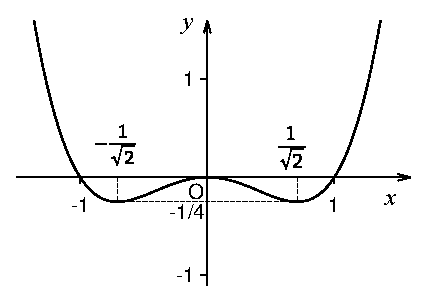
\includegraphics[width=7cm]{xxxx_xx.eps}
    \caption{$y=x^4-x^2$のグラフ(実線)。\label{fig:xxxx_xx}}
\end{figure}

\begin{exmpl} $y=x^4-x^2$のグラフを描いてみよう。まずこれは偶関数である。
また, $x$軸との共有点($y=0$)は, $x=0, \pm 1$である。

次に極大と極小を求める。$f'(x)=4x^3-2x$だから, $x=0, \pm 1/\sqrt{2}$で
$f'(x)=0$となる。それぞれ極大・極小のどちらだろう?

$x=-1/\sqrt{2}$については, それより少し小さな$x$では$f'(x)<0$ (つまり$f(x)$は減少傾向), それより
少し大きな$x$では$f'(x)>0$ (つまり$f(x)$は増加傾向)となるから, そこでは
極小値$f(-1/\sqrt{2})=-1/4$をとる。$x=1/\sqrt{2}$についても同様である。

一方, $x=0$については, それより少し小さな$x$では$f'(x)>0$ (つまり$f(x)$は増加傾向), 
それより少し大きな$x$では$f'(x)<0$ (つまり$f(x)$は減少傾向)となるから, そこでは
極大値$f(0)=0$をとる。

$x\rightarrow\infty$で$f(x)\rightarrow\infty$であることを併せて
考えると, 図\ref{fig:xxxx_xx}のようなグラフになる。(例おわり)\end{exmpl}


以上でわかったように, なめらかな関数のグラフが極大値や極小値をとる場所では, 
微分係数は0である。しかし, その逆は必ずしも成り立たないことに注意しよう。
つまり, 微分係数が0であっても, 極大にも極小にもならない, という場合が
存在するのだ。\mv

\begin{exmpl}
$y=x^3$は$x=0$での微分係数は0だが, P.\pageref{fig:xxx-x}の
図\ref{fig:xxx-x}の点線で示されるように, $y=x^3$の
グラフは, $x=0$で極大にも極小にもならない。
(例おわり)\end{exmpl}
\vv




\section{偶関数や奇関数の微分}

関数$f(x)$が偶関数であるとする。すなわち, $f(-x)=f(x)$が恒等的に成り立つ。
この両辺を$x$で微分すると, $-f'(-x)=f'(x)$となる(左辺は合成関数の微分!)。
すなわち, $f'(-x)=-f'(x)$が恒等的に成り立つ, すなわち$f'(x)$は奇関数
である。偶関数の導関数は奇関数なのだ!

\begin{comment}
その導関数を$f'(x)$とすると, \eref{eq:define_dif10}より, 
\begin{eqnarray}f'(x)=\frac{f(x+dx)-f(x)}{dx}\label{eq:diff_evenfunc0}\end{eqnarray}
である。この式で, 形式的に, $x$を$-x$に, $dx$を$-dx$に書き換えると
\begin{eqnarray}f'(-x)=\frac{f(-x-dx)-f(-x)}{-dx}\end{eqnarray}
となるが, $f(x)$は偶関数なので, 
\begin{eqnarray}f(-x)=f(x),\,\,\, f(-x-dx)=f(x+dx)\end{eqnarray}
なので, 
\begin{eqnarray}
f'(-x)&=&\frac{f(x+dx)-f(x)}{-dx}\\
      &=&-\frac{f(x+dx)-f(x)}{dx}=-f'(x)\end{eqnarray}
従って, $f'(x)$は奇関数である。

\begin{freqmiss}{\small\textgt{上の論証過程で, 「$x=-x$, $dx=-dx$とすると」
と書いてしまう} ... もし$x=-x$なら, 右辺を左辺に移項して$2x=0$, 従って$x=0$
となってしまう! 同様に, $dx=0$となってしまう! $x=-x$と書きたい気持ちは
わからなくもないですが, ひとつの等式の中に現れる以上は, 左辺の$x$と右辺の$x$は
同じ数として扱わざるを得ません。そもそも, \eref{eq:diff_evenfunc0}
はどんな$x$にも成り立つから, 「$x$のところを$-x$と書きなおしてもよかろう」
と考えるのだけど, それを$x=-x$と書いてしまうのは乱暴です。}\end{freqmiss}

\begin{freqmiss}{\small\textgt{上の論証過程で, 「$dx$を$-dx$に」という
部分を省略してしまう} ... そうしたい気持ちはわからなくもないですが, $x$と$dx$は
別の量。$x$を$-x$に置き換えたからといって, $dx$も自動的に$-dx$に
置き換わるものではないのです。}\end{freqmiss}
\hv
\end{comment}

%------------
\begin{q}\label{q:diff_odd} 奇関数の導関数は偶関数であることを示せ。\end{q}
\mv

%------------
\begin{q}\label{q:diff_oddeven} $n$を0以外の任意の整数とする。
以下の関数について, 偶関数の導関数が奇関数になり, 
奇関数の導関数が偶関数になることを実際に確認せよ。なお, 
単に「確認した」というだけではレポートにはなりません!
\begin{edaenumerate}
\item $f(x)=x^{2n}$
\item $f(x)=x^{2n+1}$
\item \begin{eqnarray*}f(x)=\frac{1}{1+x^2}\end{eqnarray*}
\item \begin{eqnarray*}f(x)=\frac{x}{1+x^2}\end{eqnarray*}
\end{edaenumerate}\end{q}
ヒント: (3), (4)は問\ref{q:diff_func5}に出てきた。\mv

%\begin{q}\label{q:differential_English} 以下の言葉を英訳せよ:
%\begin{edaenumerate}<3>
%\item 微分する
%\item 導関数
%\item 変位
%\item 距離
%\item 速さ
%\item 速度
%\item 加速度
%\end{edaenumerate}
%\end{q}\mv

%\section*{一問一答}
%\begin{itemize}\item 無限大×無限小は?\end{itemize}
% 場合によります。$x$が無限大になるときには, $x\times(1/x)$や$x^2\times(1/x)$, 
%$x\times(1/x^2)$などは, いずれも「無限大×無限小」になりますが, 最初のは1になり, 
%2番めのは無限大になり, 最後のは0になります。

%\section*{一問一答}

%\begin{itemize}
%\item はじめて微分係数を考えた人はすごいと思った。
%\end{itemize}
% ニュートンとかライプニッツだと言われていますが, 実はそれより前に, 
%江戸時代の日本の数学者である関孝和も微分に近い概念を発見したそうです。関孝和には多くの
%素晴らしい業績があります。

%\begin{itemize}
%\item 微分の$f'(x)$の「'」は誰が決めたんですか?
%\end{itemize}
% ラグランジュです。$df/dx$という書き方はライプニッツが決めました。君が習う
%数学は, 物理学とともに18世紀〜19世紀頃に大きく発展した内容です。そこには何人かの
%スーパースターがいます。ラグランジュ, ライプニッツ, ニュートン, ガウス, オイラー, 
%コーシー, ラプラス, ダランベール等という名前は, これから何回も目にするでしょう。
%ちなみにラグランジュはマリー・アントワネットの数学教師だったそうです。


\begin{faq}\small{\textgt{数IIIをやっていないのでテストができません。}
... もう高校時代は終わったのだから「XXXをやって
いないから」というのはやめましょう。やっていなければ, 今, やればいいのです。
高校で数IIIをやった人も, それなりの苦労や努力をしたのです。}\end{faq}
\hv



\section*{演習問題}


\begin{exq} 
\begin{enumerate}
\item $y=1/x^n$と置き, その両辺を$x^n$倍し, その両辺を$x$で微分する, 
という発想で, \eref{eq:xpowminusn1}を導け。
\item $y=x^{1/n}$と置き, その両辺を$n$乗し, その両辺を$x$で微分する, 
という発想で, \eref{eq:xpowfrc}を導け。
\end{enumerate}
\end{exq}

\begin{exq} 逆関数の微分の公式 (\eref{eq:diff_form5})を, グラフの「接線の傾き」
という観点で示せ。ヒント: 逆関数のグラフは, もとの関数を, 
直線$y=x$に関して対称移動したもの。\end{exq}

\begin{exq}\label{q:diff_Legendre} $n$を0以上の整数とするとき, 以下の式で定義される
関数$P_n(x)$をルジャンドル関数\index{るじゃんどるかんすう@ルジャンドル関数}という
\footnote{この関数は, 実は原子の電子軌道(K殻とかL殻とか)
と密接な関係がある。}
\begin{eqnarray}
P_n(x) :=\frac{1}{2^n n!}\,\frac{d^n}{dx^n}(x^2-1)^n
\end{eqnarray}
\begin{enumerate}
\item $n=0, 1, 2, 3, 4$のそれぞれについて, $P_n(x)$を求めよ。
%\item $n=0, 1, 2, 3, 4$のそれぞれについて, $P_n(1)=1$であることを示せ。
\item $n$が偶数のときは$P_n(x)$は偶関数であることを示せ。
\item $n$が奇数のときは$P_n(x)$は奇関数であることを示せ。
\end{enumerate}
\end{exq}
\vv

\section*{問題の解答}

%\noindent{\textbf{答}}\ref{q:diff_def00} 略 (がんばれ!)\mv

%
\noindent{\textbf{答}}\ref{q:diff_def0}  無限小$dx$に対して, 
$g(a+dx) = g(a)+g'(a)dx$
と書けるとき, 右辺の$dx$の係数$g'(a)$のこと。もしくは, 
\begin{eqnarray*}g'(a)=\lim_{\Delta x \to 0} \frac{g(a+\Delta x)-g(a)}{\Delta x}\end{eqnarray*}
のこと(どちらでも可)。{\small 注: この問題で, あなたは
$g$を$f$と書いたり$a$を$x_0$と書いたりしなかっただろうか? 
本文に出てきた$f(x)$や$x_0$という記号は, 説明のための
便宜的なものであり, この問題のように, 設定に応じて変わるものである。}
\mv

%
\noindent{\textbf{答}}\ref{q:diff_const} 
\begin{eqnarray*}
f(x+dx)&=&p(x+dx) + q=px+q+p\,dx\\
       &=&f(x)+p\,dx
\end{eqnarray*}
$dx$の係数に着目して, $f'(x)=p$。
特に, $f(x)$が定数関数の場合は$p=0$だから, 
$f'(x)$は恒等的に0。\qed
\mv

% 表計算ソフトで, 関数$f(x)=x^2$を, $-2 \le x \le 2$の範囲で数値微分し, 
%\noindent{\textbf{答}}\ref{q:comp_diff0} 略。\mv

% 以下の関数を微分せよ:
\noindent{\textbf{答}}\ref{q:diff_func0}
\begin{edaenumerate}
\item $f'(x)=2x+1$
\item $f'(x)=8x+5$
\item $f'(x)=6x+3$
\item $f'(x)=-5/x^2$
\item $f'(x)=1+1/x^2$
\end{edaenumerate}

% 以下の関数:\begin{eqnarray}f(x)=(x^2+x+1)(x^2-x-2)\end{eqnarray}について, 
\noindent{\textbf{答}}\ref{q:diff_func1}
\begin{eqnarray*}
(1)\quad f'(x)&=&(x^2+x+1)'(x^2-x-2)\\
     &+&(x^2+x+1)(x^2-x-2)'\\
     &=&(2x+1)(x^2-x-2)\\
     &+&(x^2+x+1)(2x-1)\\
     &=&4x^3-4x-3\\
(2)\quad f(x)&=&x^4-2x^2-3x-2\\
f'(x)&=&4x^3-4x-3
\end{eqnarray*}

% 以下の関数を, 合成関数の微分の公式を使って微分せよ:
\noindent{\textbf{答}}\ref{q:diff_func2}
\begin{enumerate}
\item ($g(x)=x^3$, $f(x)=3x^2+2$とみなせばよい。)
\begin{eqnarray*}
F'(x)&=&3(3x^2+2)^2(3x^2+2)'\\
     &=&3(3x^2+2)^2(6x)=18x(3x^2+2)^2\end{eqnarray*}
\item ($g(x)=x^3$, $f(x)=x^2+x+1$とみなせばよい。)
\begin{eqnarray*}
F'(x)&=&3(x^2+x+1)^2(x^2+x+1)'\\
     &=&3(x^2+x+1)^2(2x+1)
\end{eqnarray*}
\item ($g(x)=x^2, f(x)=x^5+x^4+x^3+x^2+x+1$とみなせばよい。)
\begin{eqnarray*}
F'(x)=2&(x^5+x^4+x^3+x^2+x+1)\\
       &\,\,\times(x^5+x^4+x^3+x^2+x+1)'\\
     =2&(x^5+x^4+x^3+x^2+x+1)\\
       &\,\,\times(5x^4+4x^3+3x^2+2x+1)
\end{eqnarray*}
\item ($g(x)=x^2$, $f(x)=1+1/x$とみなせばよい。)
\begin{eqnarray*}
F'(x)&=&2\Bigl(1+\frac{1}{x}\Bigr)\Bigl(1+\frac{1}{x}\Bigr)'\\
     &=&-2\Bigl(1+\frac{1}{x}\Bigr)\frac{1}{x^2}=-2\Bigl(\frac{1}{x^2}+\frac{1}{x^3}\Bigr)
\end{eqnarray*}
\end{enumerate}

% 関数$g(x)$の逆数であらわされる関数$1/u(x)$の導関数は, 以下で与えられることを示せ:
\noindent{\textbf{答}}\ref{q:diff_func3} 関数$1/u(x)$は, 関数$1/x$と関数$u(x)$の合成関数である。$(1/x)'=-1/x^2$だから, 
\begin{equation*}
\Bigl(\frac{1}{u}\Bigr)'=\Bigl(-\frac{1}{u^2}\Bigr)u'=-\frac{u'}{u^2}
\end{equation*}

% 関数$f(x)$と$u(x)$の比で作られる関数$f(x)/u(x)$の導関数は, 以下で与えられることを示せ:
\noindent{\textbf{答}}\ref{q:diff_func4} 関数$v(x)/u(x)$は, 関数$v(x)$と関数$1/u(x)$の積である。
\begin{eqnarray*}
\Bigl(v\times\frac{1}{u}\Bigr)'&=&v'\Bigl(\frac{1}{u}\Bigr)+v\Bigl(\frac{1}{u}\Bigr)'\\
&=&v'\Bigl(\frac{1}{u}\Bigr)+v\Bigl(-\frac{u'}{u^2}\Bigr)=\frac{v'u-vu'}{u^2}
\end{eqnarray*}

% 以下の関数を微分せよ:
\noindent{\textbf{答}}\ref{q:diff_func5}
\begin{edaenumerate}
\item \begin{eqnarray*}-\frac{2x}{(1+x^2)^2}\end{eqnarray*}
\item \begin{eqnarray*}\frac{1-x^2}{(1+x^2)^2}\end{eqnarray*}
\end{edaenumerate}

% べき関数の微分の公式を使って, 以下の関数を微分せよ。
\noindent{\textbf{答}}\ref{q:diff_pow} 
\begin{edaenumerate}
\item \begin{eqnarray*}-\frac{1}{x^2}\end{eqnarray*}
\item \begin{eqnarray*}-\frac{1}{2x^{3/2}}=-\frac{1}{2}x^{-3/2}\end{eqnarray*}
\item \begin{eqnarray*}\frac{2}{3}x^{-1/3}\end{eqnarray*}
\item \begin{eqnarray*}-5x^{-6}\end{eqnarray*}
\end{edaenumerate}

% 微分の公式1〜5を証明せよ。
%\noindent{\textbf{答}}\ref{q:diff_theories1_5} 略(本文参照)。\hv

% 以上の微分の公式を駆使して, 以下の関数を微分せよ:
\noindent{\textbf{答}}\ref{q:diff_func8}
\begin{enumerate}
\item ヒント: $g(x)=\sqrt{x}$, $f(x)=2x+3$として公式4を使う。$g'(x)=1/(2\sqrt{x})$だから, 
\begin{eqnarray*}\text{(与式)}'=\frac{f'(x)}{2\sqrt{f(x)}}=\frac{(2x+3)'}{2\sqrt{2x+3}}=\frac{2}{2\sqrt{2x+3}}\\
=\frac{1}{\sqrt{2x+3}}\end{eqnarray*}
\item ヒント: $g(x)=\sqrt{x}$, $f(x)=1-x^2$として公式4を使う。$g'(x)=1/(2\sqrt{x})$だから, 
\begin{eqnarray*}\text{(与式)}'=\frac{f'(x)}{2\sqrt{f(x)}}=\frac{(1-x^2)'}{2\sqrt{1-x^2}}=\frac{-2x}{2\sqrt{1-x^2}}\\
=-\frac{x}{\sqrt{1-x^2}}\end{eqnarray*}
\item ヒント: まず$x^2$と$\sqrt{1+x^2}$の積と考えて公式3を使う。その上で例\ref{exmpl:diff_sqrtx2p1}を使う。
\begin{eqnarray*}\text{(与式)}'=(x^2)'\sqrt{1+x^2}+x^2(\sqrt{1+x^2})'\\
=2x\sqrt{1+x^2}+\frac{x^3}{\sqrt{1+x^2}}\end{eqnarray*}
\item ヒント: $g(x)=x^{-1/2}$, $f(x)=1+x^2$として公式4を使う。
\begin{eqnarray*}&&\text{(与式)}'=\frac{-1}{2}(f(x))^{-3/2}f'(x)\\
&&=\frac{-1}{2}(1+x^2)^{-3/2}(2x)=-\frac{x}{(1+x^2)^{3/2}}\end{eqnarray*}
\item ヒント: $g(x)=1/x$, $f(x)=1+\sqrt{x}$として公式4を使う。
\begin{eqnarray*}&&\text{(与式)}'=-\frac{(1+\sqrt{x})'}{(1+\sqrt{x})^2}\\
&&=-\frac{\frac{1}{2\sqrt{x}}}{(1+\sqrt{x})^2}=-\frac{1}{2\sqrt{x}(1+\sqrt{x})^2}\end{eqnarray*}
\item ヒント: $g(x)=\sqrt{x}$, $f(x)=1+1/x$として公式4を使う。
\begin{eqnarray*}\text{(与式)}'
=\frac{1}{2\sqrt{1+\frac{1}{x}}}\Bigl(1+\frac{1}{x}\Bigr)'=\frac{-1}{2x^2\sqrt{1+\frac{1}{x}}}\end{eqnarray*}
\item ヒント: $x-1$と$1/(x+1)$の積と考えて公式3を使う。
\begin{eqnarray*}\text{(与式)}'=(x-1)'\frac{1}{x+1}+(x-1)\Bigl(\frac{1}{x+1}\Bigr)'\\
=\frac{1}{x+1}-(x-1)\frac{1}{(x+1)^2}=\frac{2}{(x+1)^2}\end{eqnarray*}
別解: 与式=$1-2/(x+1)$と変形してから微分しても, 同じ結果になる。
\item ヒント: $g(x)=1/x$, $f(x)=1+1/x$として公式4を使ってもよいのだが, 
与式を変形してから微分するほうが簡単。与式の分母分子に$x$をかけて, 
\begin{eqnarray*}\text{(与式)}=\frac{x}{x+1}=1-\frac{1}{x+1}\end{eqnarray*}
従って, 
\begin{eqnarray*}\text{(与式)}'=\Bigl(1-\frac{1}{x+1}\Bigr)'=\frac{1}{(x+1)^2}\end{eqnarray*}
\end{enumerate}
\hv


% 解答: 線型近似
\noindent{\textbf{答}}\ref{q:univ_lin_approx0}  \
$f(x)=(1+x)^a$と置くと, $f(0)=1$。また, $f'(x)=a(1+x)^{a-1}$なので, 
従って$f'(0)=a$。これを\eref{eq:linear_approx00}に入れると, 与式を得る。\mv

\noindent{\textbf{答}}\ref{q:univ_lin_approx2}  \
\begin{enumerate}
\item \eref{eq:linear_approx02}で$a=-1$とすれば, $1/(1+x)\fallingdotseq1-x$
\item 前小問の$x$を$-x$に置き換えて, $1/(1-x)\fallingdotseq1+x$
\item \eref{eq:linear_approx02}で$a=-1/2$とすれば, \\$1/\sqrt{1+x}\fallingdotseq1-x/2$
\end{enumerate}
\mv

\noindent{\textbf{答}}\ref{q:univ_lin_approx4} 
\begin{enumerate}
\item $(0.99)^{10}=(1-0.01)^{10} \fallingdotseq 1-10 \times 0.01=0.9$
\item 3乗して10に近い簡単な数は何かな?と考えると, 2が思いつく。$2^3=8$であることに
注目し, 
\begin{eqnarray*}
10^{1/3}&=&(8+2)^{1/3}=\Bigl\{8\Bigl(1+\frac{2}{8}\Bigr)\Bigr\}^{1/3}\\
&=&8^{1/3}\Bigl(1+\frac{2}{8}\Bigr)^{1/3}=2\Bigl(1+\frac{1}{4}\Bigr)^{1/3}\\
&\fallingdotseq&2\Bigl(1+\frac{1}{3\times4}\Bigr)=2+\frac{1}{6}=2.166\cdots
\end{eqnarray*}
\end{enumerate}
\mv

% 以下の関数について, $f'(x)$, $f''(x)$, $f^{(3)}(x)$をそれぞれ求めよ。
\noindent{\textbf{答}}\ref{q:diff_func9}
\begin{edaenumerate}
\item
\begin{eqnarray*}
&&f'(x)=5x^4+6x^2\\
&&f''(x)=20x^3+12x\\
&&f^{(3)}(x)=60x^2+12
\end{eqnarray*}
\item
\begin{eqnarray*}
&&f'(x)=\frac{1}{(1-x)^2}\\
&&f''(x)=\frac{2}{(1-x)^3}\\
&&f^{(3)}(x)=\frac{6}{(1-x)^4}
\end{eqnarray*}
\end{edaenumerate}

% $n$を0以上の整数とするとき, 以下の式で定義される
%\noindent{\textbf{答}}\ref{q:diff_Legendre}
%\begin{eqnarray*}
%P_0(x)&=&\frac{1}{2^00!}(x^2-1)^0=1\\
%P_1(x)&=&\frac{1}{2^11!}(x^2-1)'=\frac{2x}{2}=x\\
%P_2(x)&=&\frac{1}{2^22!}\{(x^2-1)^2\}''=\frac{(x^4-2x^2+1)''}{8}\\
%      &=&\frac{12x^2-4}{8}=\frac{3x^2-1}{2}\\
%P_3(x)&=&\frac{1}{2^33!}\{(x^2-1)^3\}'''=\frac{(x^6-3x^4+3x^2-1)'''}{48}\\
%      &=&\frac{120x^3-72x}{48}=\frac{5x^3-3x}{2}
%\end{eqnarray*}
%\hv

\noindent{\textbf{答}}\ref{q:diff_def} (1), (2), (3)は略。
本文をよく読めば簡単。(4) 「距離を」ではなく「位置を」と言わねばならない。距離を
時刻で微分したものは「速さ」である。(5) 間違っているとは言い切れないが, 
「時刻によって微分」と言わねば不正確である。\mv

% 点Pが, $x$軸上を運動している。時刻$t$のときPの位置が$x=t^2-3t+1$と書けるとき
\noindent{\textbf{答}}\ref{q:diff_velocac} (1) 位置を時刻で微分する: $(at^2+bt+c)'=2at+b$。
(2) 再度時刻で微分する: $(2at+b)'=2a$。\mv

\noindent{\textbf{答}}\ref{q:diff_velocac1} 
問\ref{q:diff_velocac}(2)で, $2a$が加速度なので, $a$は加速度の次元(SI単位ではm~s$^{-2}$)。
問\ref{q:diff_velocac}(1)で, $2at+b$が速度なので, $b$は速度の次元(SI単位ではm~s$^{-1}$)。
もともと$x=at^2+bt+c$だったので, $c$は$x$と同じ次元(長さ; SI単位ではm)。\mv

\noindent{\textbf{答}}\ref{q:diff_velocac2}(略解) 位置は503~m。速度は99~m~s$^{-1}$。
加速度は9.8~m~s$^{-2}$。\mv

\noindent{\textbf{答}}\ref{q:vect_throw} ${\bf r}(t)=(v_0t,\, -gt^2/2)=(x, y)$と置く。
(1) $x, y$から$t$を消去して, $y=-gx^2/(2v_0^2)$。これを$xy$平面にプロットすると, 
原点を頂点とする, 上に凸の放物線になる。 (2) ${\bf v}(t)={\bf r}'(t)=(v_0,\, -gt)$  
(3) ${\bf a}(t)={\bf v}'(t)=(0,\, -g)$。なお, この点の運動は, 水平方向に初速$v_0$で投げたボールの運動である。\mv


% 奇関数の導関数は偶関数であることを示せ。
\begin{comment}
\noindent{\textbf{答}}\ref{q:diff_odd} 
 関数$f(x)$が奇関数であるとする。その導関数を$f'(x)$とすると, 導関数の定義より, 
\begin{eqnarray}f'(x)=\frac{f(x+dx)-f(x)}{dx}\end{eqnarray}
である。この式で, 形式的に, $x$を$-x$に, $dx$を$-dx$に書き換えると
\begin{eqnarray}f'(-x)=\frac{f(-x-dx)-f(-x)}{-dx}\end{eqnarray}
となるが, 奇関数の定義より$f(-x)=-f(x)$, $f(-x-dx)=-f(x+dx)$なので, 
\begin{eqnarray}f'(-x)&=&\frac{-f(x+dx)+f(x)}{-dx}\nonumber\\
&=&\frac{f(x+dx)-f(x)}{dx}=f'(x)\end{eqnarray}
従って, $f'(x)$は偶関数である。\qed
\hv
\end{comment}

% 
\noindent{\textbf{答}}\ref{q:diff_oddeven} (1) $f(-x)=(-x)^{2n}=
(-1)^{2n}x^{2n}=x^{2n}=f(x)$。よって$f(x)$は偶関数。$f'(x)=2nx^{2n-1}$。
$f'(-x)=2n(-x)^{2n-1}=(-1)^{2n-1}2nx^{2n-1}=-2nx^{2n-1}=-f'(x)$。
よって$f'(x)$は奇関数。(2)以下略。

\begin{comment}
図\ref{fig:even_odd_function}参照。
\begin{figure}[h]
    \centering
    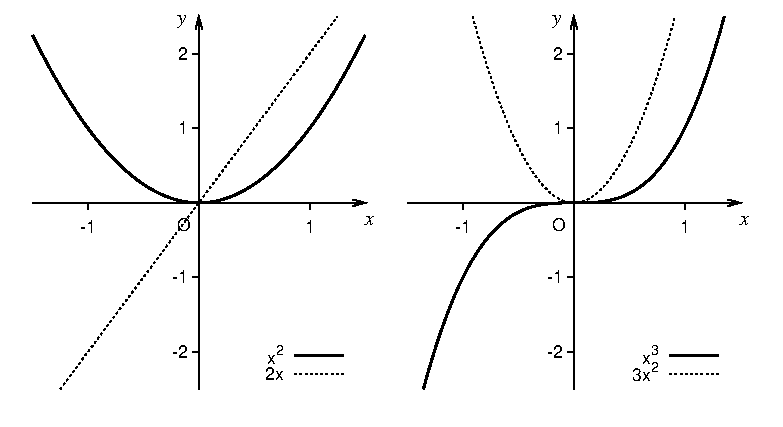
\includegraphics[width=8cm]{even_odd_function.eps}
    \caption{左:$y=x^2$(実線)と$y=2x$(破線)のグラフ。右:$y=x^3$(実線)と$y=3x^2$(破線)のグラフ。}\label{fig:even_odd_function}
\end{figure}
\end{comment}

